\chapter{Theoretical framework}
\label{chapter:Theory}

The Standard Model (SM) of particle physics is the theoretical framework that so far describes best the subatomic world. Since its development the 1960's, it has been thoroughly tested and has been very successful in describing experimental observations. In addition, all the predicted phenomena have found experimental confirmation, the last one being the observation of the Higgs boson at the Large Hadron Collider in July 2012~\cite{Aad:2012tfa,Chatrchyan:2012ufa}.

This chapter introduces the building blocks of the SM, its experimental successes and shortcomings, and a summary of theories beyond the SM. The phenomenology of these theories is detailed, with emphasis on their collider signatures.

\section{The Standard Model}
\label{sec:IntroSM}

The Standard Model (SM) of particle physics \cite{Glashow:1961tr, Weinberg:1967tq, Salam:1980jd} is a renormalizable quantum field theory based on the total invariance under the gauge group:

\begin{equation}
  SU(3)_{C}\otimes SU(2)_{L}\otimes U(1)_{Y}~,
  \label{eq:SMSymmetryGroup}
\end{equation}
where $SU(3)_{C}$ is the symmetry group of the strong interaction and $SU(2)_{L}\otimes U(1)_{Y}$ corresponds to the electroweak interaction.

The SM describes the interaction among the constituents of matter, \textit{fermions}, through the exchange of force mediators, \textit{bosons}. 
More precisely, the SM describes particles as field functions of space-time coordinates. % $\varphi(x)$. 
%The dynamics of the fields are described with a lagrangian density, \lagrangian:
Fermions are described as spin-1/2 Dirac fields, satisfying the lagrangian:
%, which is a function of the field and it first derivatives ∂µϕ(x):
%\begin{equation}
%  \lagrangian\left(\varphi(x),\partial\varphi(x)\right)
%  \label{eq:Lagrangian}
%\end{equation}
\begin{equation}
  \lagrangian = \bar{\psi}(i\gamma^{\mu}\partial_\mu -m)\psi~,
  \label{eq:QEDLagrangianGlobalInvariant}
\end{equation}
where $\psi$ is the fermion field, $\gamma^{\mu}$ are the Dirac matrices and $m$ is the mass of the fermion.

Imposing the lagrangian to be invariant under local transformations of a given symmetry group requires the introduction
of gauge fields (boson fields). 
The number of associated boson fields is equal to the number of generators of the symmetry group. 
In the SM, the gauge symmetry $SU(3)_{C}$ determines the strong interaction
mediated by gluons, while the {$SU(2)_{L}\otimes U(1)_{Y}$} gauge symmetry
governs the electroweak interaction mediated by the photons, $W^{\pm}$ and $Z$ bosons.
%The mathematical description of the interactions arises from requiring the invariance of the Lagrangian under a local gauge transformation of given symmetry group. The requirement of gauge invariance leads to a conserved quantity, and to the introduction of a number of gauge bosons, which only interact with fields carrying the conserved charge.
%The number of vector bosons, the type of conserved charge and the nature of the interaction depend on the symmetry group the gauge transformation belongs to.
Table~\ref{tab:bosons} summarizes the classification of bosons in the SM.

\begin{table}[!ht]
  \begin{center}
    \begin{tabular}{lccc}
        \toprule
        \toprule
        Mediator               & Mass [\gev]     & Interaction & Electric charge \\
        \midrule
        Gluon ($\times 8$) $(g)$     & 0                    & Strong            & 0                     \\
        Photon ($\gamma$)            & 0                    & Electromagnetic   & 0                     \\
        $Z$                          & 91.19                & Weak              & 0                     \\
        $W^{\pm}$                    & 80.39                & Weak              & $\pm 1$               \\
        \bottomrule
        \bottomrule
      \end{tabular}
  \end{center}
  \caption{Table of gauge bosons in the SM with their mass and charge according to the Particle Data Group~\cite{PDG}.}
  \label{tab:bosons}
\end{table}


The bosonic sector of the SM is responsible for three of the four interactions in Nature.
Gravity can not be accommodated since a renormalizable formulation as a quantum field theory is not known, thus being one of the motivations to look for physics beyond the SM.
\newline

Fermions are classified in quarks and leptons, and subdivided in three families or generations. 
Generations of quarks and leptons are copies with the same quantum numbers except for their masses, 
having the 1\textsuperscript{st} generation the lighter particles and the 3\textsuperscript{rd} the heavier. 
Table \ref{tab:QuarksAndLeptons} provides a classification of the SM fermions.

\begin{table}[b!]
  \begin{center}
      \begin{tabular}{ccccc}
        \toprule
        \toprule
        Generation & Name & Symbol & Mass & Electric charge  \\
        \midrule
        \multicolumn{5}{c}{{\bf Quarks}} \\
        \midrule
        \multirow{2}{*} {$1^\text{st}$} & Up     & $u$ & \unit[2.3]{\mev}     & $+2/3$ \\
        & Down   & $d$ & \unit[4.8]{\mev}     &$-1/3$ \\
        \\
        \multirow{2}{*} {$2^\text{nd}$} & Charm  & $c$ & \unit[1.275]{\gev}   & $+2/3$ \\
        & Strange& $s$ & \unit[95]{\mev}      &$-1/3$ \\
        \\
        \multirow{2}{*} {$3^\text{rd}$} & Top    & $t$ & \unit[173.5]{\gev}  & $+2/3$ \\
        & Bottom & $b$ & \unit[4.65]{\gev}    &$-1/3$ \\
        \midrule
        \multicolumn{5}{c}{{\bf Leptons}} \\
        \midrule
        \multirow{2}{*} {$1^\text{st}$} & Electron           & $e$ & \unit[0.51]{\mev} & -1\\
        & Electron neutrino  & $\nu_e$    & $<$ \unit[2]{eV} & 0\\
        \\
        \multirow{2}{*} {$2^\text{nd}$} & Muon               & $\mu$ &\unit[105.66]{\mev} & -1\\
        & Muon neutrino      & $\nu_{\mu}$ & $<$ \unit[2]{eV} & 0\\
        \\
        \multirow{2}{*} {$3^\text{rd}$} & Tau                & $\tau$   & \unit[1.77]{\gev} & -1 \\
        & Tau neutrino       & $\nu_{\tau}$& $<$ \unit[2]{eV} & 0\\
        \bottomrule
        \bottomrule
      \end{tabular}
    \caption{Table of quark and lepton families with their mass and charge according to the Particle Data Group~\cite{PDG}.
    \label{tab:QuarksAndLeptons}}
  \end{center}
\end{table}

Additionally, for each quark and lepton exists an anti-particle, thus doubling the number of fermions.
The anti-particles are characterized by having the same masses but opposite quantum numbers.

In order to study the SM lagrangian one can proceed by splitting the lagrangian in two terms: 
one describing electroweak interactions, and a second one describing quantum chromodynamics (QCD).
%one including the strong sector described with the quantum chromodynamics (QCD) theory, and a second one for the electroweak sector, which unifies electromagnetic
%and weak interactions.
\begin{equation}
  \lagrangian_{SM} = \lagrangian_{EW} + \lagrangian_{QCD}
  \label{eq:LagrangianSplit}
\end{equation}

\subsection{Electroweak theory}
\label{subsec:EW}

The electroweak theory describes the weak and the electromagnetic interactions. It unifies the forces in the symmetry group $SU(2)_{L}\otimes U(1)_{Y}$.
The symmetry group of the weak interaction is the $SU(2)_{L}$ group, and a new quantum number, referred to as weak isospin, $T$, is introduced. 
The generators of the group are the weak isospin operators, $\hat{T}_i = \frac{\sigma_i}{2}\;(i=1, 2, 3)$, where $\sigma_i$ are the three Pauli matrices.
The left- and right-handed components of the fermion fields:
\begin{align}
  \begin{split}
    \psi_L &= \frac{1}{2}\left(1-\gamma^5\right)\psi \\
    \psi_R &= \frac{1}{2}\left(1+\gamma^5\right)\psi~,
  \end{split}
  \label{eq:chirality_projection}
\end{align}
transform differently under the operators of the weak symmetry group.
Left-handed fermions transform as doublets,
%under the weak isospin operators, 
whereas right-handed fermions transform as singlets:
  %anti-particles in the opposite way.

\begin{equation}
  \begin{split}
    f_L^i = \left(
    \begin{matrix}
      \nu_L^i \\
      \ell_L^i
    \end{matrix} \right) ,\;
    \left(
    \begin{matrix}
      u_L^i \\
      d_L^i
    \end{matrix} \right) \\
    f_R^i = \ell_R^i,\; u_R^i,\; d_R^i,
  \end{split}
  \label{eq:EWKmultiplets}
\end{equation}
where $i=1,2,3$ is the family (generation) index. The subscript in $SU(2)_{L}$ refers to the fact that only the left-handed fermions interact through the weak force.

The second part of the symmetry group, $U(1)_Y$, introduces a new conserved quantum number, $Y$, the hypercharge.
The electric charge is  related to the third component of the weak isospin $T_3$ and the hypercharge $Y$ by the Gell-Mann Nishijima formula:

\begin{equation}
  \hat{Q} = \hat{T}_3 + \frac{\hat{Y}}{2}~.
  \label{eq:ElectricChargeDefinition}
\end{equation}

In order to respect local invariance under both symmetry groups, the covariant derivative is introduced in equation~\ref{eq:QEDLagrangianGlobalInvariant}:

\begin{equation} 
  D_\mu \equiv \partial_\mu - ig\vec{T}\cdot\vec{W}_\mu - ig'\frac{Y}{2}B_\mu~,
  \label{eq:EWKCovariantDerivative}
\end{equation}
where $g$ and $g'$ are the coupling constants of the $SU(2)_L$ and $U(1)_Y$ gauge groups respectively, and $\vec{W}_\mu$, $B_\mu$, are the gauge fields of the respective symmetry groups.

A kinetic term for the gauge fields has to be added to the lagrangian, in the form:

\begin{equation}
  \lagrangian_{\text{gauge}} = -\frac{1}{4}W_{\mu\nu}^i W^{\mu\nu}_i - \frac{1}{4}B_{\mu\nu}B^{\mu\nu},
  \label{eq:EWKLagrangianGauge}
\end{equation} 
where $i=1, 2, 3$, and $W_{\mu\nu}^i$ and $B_{\mu\nu}$ are the field tensors for the $SU(2)_L$ and $U(1)_Y$ gauge groups, defined as:

\begin{equation}
  \begin{split}
    W_{\mu\nu}^i & \equiv \partial_\mu W_\nu^i - \partial_\nu W_\mu^i + g\epsilon^{ijk} W_\mu^j W_\nu^k  \\
    B_{\mu\nu} & \equiv \partial_\mu B_\nu - \partial_\nu B_\mu~,
  \end{split}
  \label{eq:EWKFieldTensors}
\end{equation}
where $\epsilon^{ijk}$ is the totally antisymmetric Levi-Civita tensor, and the corresponding term is the origin of the non-abelian nature of the weak interaction.


The electroweak lagrangian can finally be written as:
\begin{equation} 
  \lagrangian_{EW} = \sum_{f=l,q}{\bar{f} \, i\gamma^\mu D_\mu \,f} + \lagrangian_{\text{gauge}}~.
  \label{eq:EWKLagrangianNoHiggs}
\end{equation}

The introduction of a mass term for either the fermions or the gauge fields breaks the local $SU(2)_L$ gauge invariance of the lagrangian,
which is not in agreement with experimental observations which point to massive vector bosons. 
Breaking gauge invariance would spoil the renormalizability of the SM, therefore a mechanism for generating non-zero masses while preserving the renormalizability of the theory needs to be introduced.

\subsection{The Higgs-Englert-Brout mechanism}
\label{sec:HiggsMechanism}

The apparent contradiction between massive particles and the requirement of gauge invariance can be solved
through a Spontaneous Symmetry Breaking (SSB), where the symmetry group $SU(2)_L \otimes U(1)_Y$ breaks down to $U(1)_{EM}$.
In order to generate the SSB, a new isospin doublet of complex scalar fields, also known as Higgs field, is introduced:

\begin{equation}
  \Phi \equiv \left(
  \begin{matrix}
    \phi^{+} \\
    \phi^{0}
  \end{matrix}
  \right) ,
  \label{eq:HiggsFieldRaw}
\end{equation}
where the ``+'' and ``0'' indices indicate the electric charge of the field.

Additional kinetic and potential terms for this new field can be added to the electroweak lagrangian in equation~\ref{eq:EWKLagrangianNoHiggs}:

\begin{equation}
  \lagrangian_{\Phi} = (D_\mu \Phi)^{\dagger} (D^\mu \Phi) - V(\Phi)~,
  \label{eq:HiggsLagrangian}
\end{equation}
where $D_\mu$ is defined in equation~\ref{eq:EWKCovariantDerivative} and:

\begin{equation}
  V(\Phi) = \mu^2 \Phi^{\dagger} \Phi + \lambda(\Phi^{\dagger} \Phi)^2~.
  \label{eq:HiggsPotential}
\end{equation}

\begin{figure}[t!]
  \centering
   \begin{subfigure}{0.47\textwidth}
  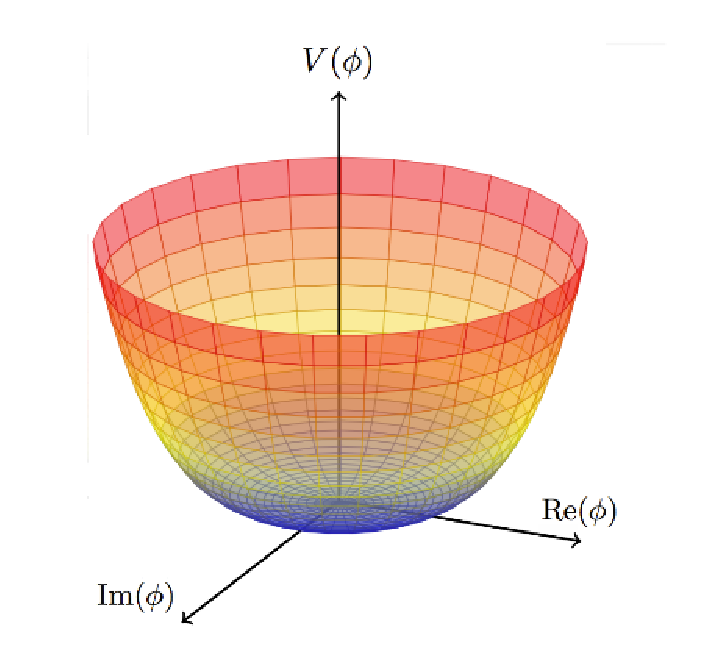
\includegraphics[width=\textwidth]{Theory/Figures/higgs1}
  \caption{}
   \end{subfigure}
   \begin{subfigure}{0.47\textwidth}
  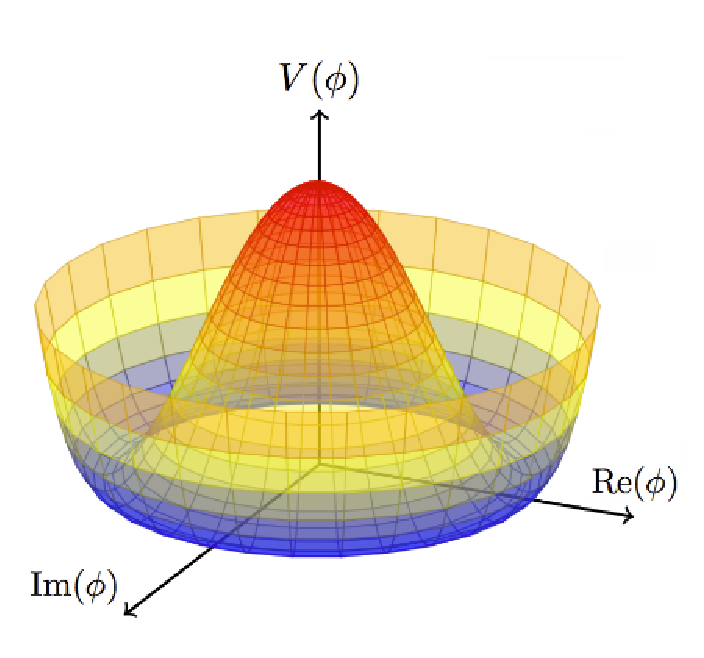
\includegraphics[width=0.9\textwidth]{Theory/Figures/higgs2}
  \caption{}
   \end{subfigure}
  \caption{Vacuum potential for $\lambda > 0$ and $\mu^2 > 0$ (a) or $\mu^2 < 0$ (b), with the typical shape of a Mexican hat.}
  \label{fig:Higgs_potential}
\end{figure}
The potential $V(\Phi)$ depends on two parameters, $\mu^2$ and $\lambda$. The case $\lambda < 0$ is unphysical, leading to no stable minima. For $\lambda > 0$, two possibilities arise: $\mu^2 > 0$ and $\mu^2 < 0$, which are illustrated in figure~\ref{fig:Higgs_potential}. In the first case there is a single solution to the minimization which corresponds to $|\Phi| =0$ and gives as vacuum expectation value (VEV), $\langle\Phi\rangle_0 \equiv \langle0|\Phi|0\rangle = 0$.
If $\lambda>0$ and $\mu^2<0$, the minimum of the potential $V(\Phi)$ is found in:

\begin{equation}
  \Phi^{\dagger} \Phi = -\frac{\mu^2}{2\lambda} \equiv \frac{v^2}{2}~,
  \label{eq:HiggsMinimumOfPotential}
\end{equation}
and therefore the field $\Phi$ has a non-zero vacuum expectation value $\langle\Phi\rangle_0 \equiv \langle0|\Phi|0\rangle = \frac{v}{\sqrt{2}}$, and there is no unique minimum. The fundamental vacuum state is no more invariant under $SU(2)_L \otimes U(1)_Y$, meaning that these two symmetries are now broken.

The Goldstone theorem states that massless scalars, referred to as Goldstone bosons, occur whenever a continuous symmetry is broken~\cite{PhysRev.127.965}.
They can be absorbed by a gauge field as a longitudinal polarization component and the gauge field acquires mass.
Since the photon is the only electroweak boson known to be massless, the minimum of the potential is chosen so that the Higgs field that acquires a VEV is the one with zero electric charge:

\begin{equation}
  \Phi_0 \equiv \frac{1}{\sqrt{2}} \left(
  \begin{matrix}
    0 \\
    v
  \end{matrix}
  \right).
  \label{eq:VEVdefinition}
\end{equation}
Expanding the field around the true minimum of the theory, the complex field $\Phi$ becomes:

\begin{equation}
  \Phi(x) = 
%e^{i\frac{\vec{\sigma}\cdot\vec{\xi}(x)}{2}} \, 
  \frac{1}{\sqrt{2}} \left(
  \begin{matrix}
    0 \\
    v + H(x)
  \end{matrix}
  \right),
  \label{eq:HiggsField}
\end{equation}
where $H(x)$ represents ground state fluctuations around the vacuum state in the direction perpendicular to the degenerate minima.
%where the three parameters $\vec{\xi}(x)$ correspond to the motion through the degenerated minima in the space, which can be set to zero ($\vec{\xi}(x)=0$) due to the gauge invariance of the lagrangian.

Additionally, nothing prevents the Higgs doublet to couple to the fermion fields.
Therefore, the interaction between the Higgs doublet and the fermion fields can be added, in the form of the Yukawa lagrangian:

\begin{equation}
  \lagrangian_{Y} = \sum_{f=l,q}{y_f \left[ \bar{f}_L \Phi f_R + \bar{f}_R \bar{\Phi}f_L \right]}~,
  \label{eq:HiggsYukawaLagrangian}
\end{equation}

\noindent where the matrices $y_f$ describe the Yukawa couplings between the Higgs doublet and the fermions.
The Yukawa lagrangian is gauge invariant since the combinations $\bar{f}_L \Phi f_R$ and $\bar{f}_R \bar{\Phi} f_L$ are $SU(2)_L$ singlets.

By introducing the expansion from equation \ref{eq:HiggsField} in the Yukawa lagrangian in equation \ref{eq:HiggsYukawaLagrangian}, the tree level predictions for the mass of the fermions can be obtained:

\begin{equation}
  m_f = y_f \frac{v}{\sqrt{2}}~,
  \label{eq:HiggsFermionMasses}
\end{equation}

\noindent where $f$ stands for the fermions of the theory.
On the other hand, the tree level mass of the Higgs boson can be computed from the Higgs lagrangian in equation \ref{eq:HiggsLagrangian}, and it is found to be:

\begin{equation}
  m_H = \sqrt{-2\mu^2} = \sqrt{2\lambda} v~.
  \label{eq:HiggsHiggsMass}
\end{equation}

Since the value of $\lambda$ is unknown, $m_H$ is not predicted by the theory and must be determined experimentally.

From the same Higgs lagrangian, the electroweak boson masses can also be obtained.
The relevant term in equation \ref{eq:HiggsLagrangian} is:

\begin{equation}
  \begin{split}
    & \left|\left(-ig\frac{\sigma}{2}\vec{W}_\mu - i\frac{g'}{2}B_\mu \right)\Phi\right|^2 \\
    &= \frac{1}{8} \left|\left(
    \begin{matrix}
      gW_\mu^3 + g'B_\mu & g(W_\mu^1 - iW_\mu^2) \\
      g(W_\mu^1 + iW_\mu^2) & -gW_\mu^3 + g'B_\mu 
    \end{matrix}
    \right)
    \left(
    \begin{matrix}
      0 \\%
      v   \
    \end{matrix}
    \right) \right|^2 \\
    &= \frac{1}{8} v^2 g^2 \left[(W_\mu^1)^2 + (W_\mu^2)^2\right] + \frac{1}{8} v^2 (g'B_\mu - gW_\mu^3)(g'B^\mu - gW^{3\mu}) \\
    &= \left(\frac{1}{2}vg\right)^2 W_\mu^{+} W^{-\mu} + \frac{1}{8} v^2 \left(W_\mu^3, B_\mu\right) 
    \left(
    \begin{matrix}
      g^2 & -gg' \\
      -gg' & g'^2
    \end{matrix}
    \right)
    \left(
    \begin{matrix}
      W_\mu^3 \\
      B_\mu
    \end{matrix}
    \right),
  \end{split}
  \label{eq:HiggsBosonMassDemonstration}
\end{equation}

\noindent defining $W^{\pm} = (W^1 \mp iW^2)/\sqrt{2}$.
The mass eigenstates can be obtained diagonalizing the mass matrix, and expressed as a function of $W_\mu^3$ and $B_\mu$:
%
%\begin{align}
%    \frac{1}{8}v^2\left[g^2\left(W_\mu^3\right)^2 - 2gg'W_\mu^3 B^\mu + g'^2B_\mu^2\right] 
%    =\ & \frac{1}{8}v^2\left[ gW_\mu^3 - g'B_\mu\right]^2           \\
%    &+ 0 \left[g'W_\mu^3 + gB_\mu\right]^2 \\
%    =\ & \frac{1}{2}\left(v\frac{\sqrt{g^2+g'^2}}2\right)^2 Z_\mu^2 & \\
%    &+ 0 \cdot A_\mu^2~, 
%  \label{eq:HiggsBosonMassDemonstration2}
%\end{align}
%
\begin{equation}
\begin{split}
    \frac{1}{8}v^2\left[g^2\left(W_\mu^3\right)^2 - 2gg'W_\mu^3 B^\mu + g'^2B_\mu^2\right] 
    =\ & \frac{1}{8}v^2\left[ gW_\mu^3 - g'B_\mu\right]^2           \\
    &+ 0 \left[g'W_\mu^3 + gB_\mu\right]^2 \\
    =\ & \frac{1}{2}\left(v\frac{\sqrt{g^2+g'^2}}2\right)^2 Z_\mu^2 \\
    &+ 0 \cdot A_\mu^2~, 
\end{split}
  \label{eq:HiggsBosonMassDemonstration2}
\end{equation}

\noindent where:

\begin{equation}
  Z_\mu = \frac{gW_\mu^3 - g'B_\mu}{\sqrt{g^2 + g'^2}}
  \label{eq:HiggsZdefinition}
\end{equation}
\begin{equation}
  A_\mu = \frac{g'W_\mu^3 + gB_\mu}{\sqrt{g^2 + g'^2}}~,
  \label{eq:HiggsAdefinition}
\end{equation}
represent the fields associated with the $Z$ boson and the photon respectively.

From equations \ref{eq:HiggsBosonMassDemonstration} and \ref{eq:HiggsBosonMassDemonstration2}, the tree level predictions for masses of the gauge bosons are:

\begin{align*}
  m_W &= \frac{vg}{2}, \\
  m_Z &= v \frac{\sqrt{g^2 + g'^2}}{2}, \\
  m_\gamma &= \unit[0]{.}
\end{align*}
%
%%\noindent By knowing that the electric charge of the photon is 0, the Nijijima equation bla bla bla can be cross-chequed.
%Finally, the Gell-Mann Nishijima formula shown in equation \ref{eq:ElectricChargeDefinition} can be validated with the boson definitions:
%
%\begin{equation}
%  \begin{split}
%    \hat{Q}A_\mu &= 0 \\
%    \hat{Q}Z_\mu &= 0 \\
%    \hat{Q}W^{\pm}_\mu &= \pm 1
%  \end{split}
%  \label{eq:ValidationElectricChargeDefinition}
%\end{equation}

\subsection{Quantum Chromodynamics}
\label{subsec:QCDtheory}

Quantum Chromodynamics (QCD) describes the strong interactions in the SM, being $SU(3)_C$  the underlying symmetry.
%responsible for the behavior of quarks being held together by the strong force, carried by gluons.
%The ``color'' group $SU(3)_C$ is the starting global symmetry.
A new quantum number, color, is introduced to refer to three different possible states of the quarks. % and it constitutes an exact symmetry of the theory.
The global gauge symmetry is promoted to a local one by introducing the covariant derivative:

\begin{equation}
  D_\mu \equiv \partial_\mu - ig_s T_a G_\mu^a~,
  \label{eq:QCDCovariantDerivative}
\end{equation}

\noindent where $g_s$ is the strong coupling constant (usually referred as $\alpha_s\equiv g_s^2 / 4\pi$ in the literature), $T_a$ are the $SU(3)_C$ generators with $a=1,\ldots,8$, and $G_\mu^a$ are the gluon fields.
After introducing the covariant derivative and a kinematic term for the gluon fields, the lagrangian of QCD is given by:

\begin{equation}
  \lagrangian_{\text{QCD}} = \bar{q}\left( i\gamma^\mu D_\mu\right) q - \frac{1}{4}G^{a}_{\mu\nu}G^{a\,\mu\nu}~,
  \label{eq:QCDlagrangian}
\end{equation}

\noindent where $\gamma^{\mu}$ are the Dirac $\gamma$-matrices and $q$ is a vector of three components corresponding to the different colors of a given quark type.
Gluons transform under the adjoint representation, while quarks are in the fundamental representation of the $SU(3)_C$ group.
The interactions between quarks and gluons are enclosed in the definition of the covariant derivative in equation \ref{eq:QCDCovariantDerivative}.
The field tensor $G^{a}_{\mu\nu}$ is given by:

\begin{equation}
  G^{a}_{\mu\nu} = \partial_{\mu}G_{\nu}^{a} - \partial_{\nu}G_{\mu}^{a} - g_s f_{abc}G_{\mu}^{b}G_{\nu}^{c}~,
  \label{eq:fieldTensorQCD}
\end{equation}

\noindent where $ f_{abc}$ are the structure constants of the $SU(3)$ group.
The third term of the tensor describes the gluon self-interaction and is responsible for the non-abelian nature of QCD.

The presence of this self-interaction induces very particular features in the dependence of the strong coupling constant with the scale of the interaction, which is shown in figure~\ref{fig:alphaRunning}. 
%The scaling of \alphas\ with $Q$ is referred to as ``running '' of the coupling constant.
\begin{figure}[tbh]
  \begin{center}
    \mbox{
      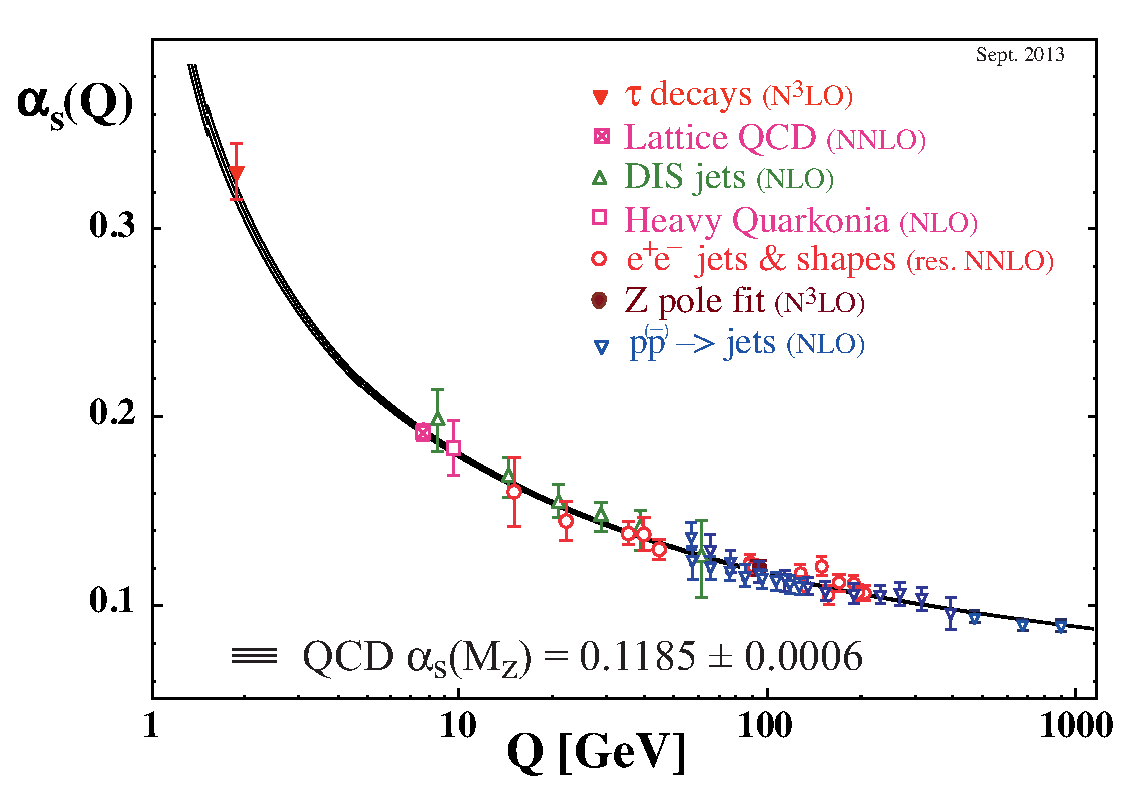
\includegraphics[width=0.7\textwidth]{Theory/Figures/asq-2013.eps}
    }
  \end{center}
  \caption{Summary of measurements of $\alpha_s$ as a function of the energy scale $Q$~\cite{Bethke:2012jm}.}
  \label{fig:alphaRunning}
\end{figure}
In the leading-order approximation~\cite{Aitchison:2004cs} the coupling constant can be expressed as:
\begin{equation}
  \alphas(Q^2)=\frac{12\pi}{(33-2n_f)\cdot \log(\frac{Q^2}{\Lambda^2_{QCD}})}~,
  \label{eq:alpha_QCD}
\end{equation}
where $n_f$ is the number of ``active flavor'' quarks (i.e. with $m_q<Q$), and $\Lambda_{QCD}$ is an infrared cut-off scale where the perturbative approximation is no longer valid. 

From equation~\ref{eq:alpha_QCD} two of the key features of QCD are derived. In the high energy regime, \alphas\ is sufficiently small that observables can be computed using perturbation theory, which gives very good mathematical properties and predictive power to the theory. Since the coupling vanishes for $Q^2 \rightarrow \infty$, in the high energy limit the quarks can propagate as if they were free, a property known as \textit{asymptotic freedom}. 
On the other hand, at low energies \alphas\ increases, to the point of diverging. This property is known as \textit{confinement}: quarks and gluons can not appear as free particles. 
When partons with colour charge start to separate from each other, the potential energy increases to a point when it becomes energetically preferable to create a quark-antiquark pair with opposite colour charge from the vacuum. This property has the experimental consequence that coloured partons  produced in high-energy interactions will manifest themselves as collimated streams of hadrons referred to as ``jets''. The process through which a quark evolves into a jet is addressed in more detail in section~\ref{subsec:HadronizationModels}.

\subsection{Experimental successes of the Standard Model}
Throughout the years the SM has been tested in multiple experiments, and its validity has been confirmed with precision measurements, sometimes with a precision better than \unit[0.1]{\%}. Since its formulation in the 70's, the SM has been able to describe accurately most experimental observations and all the discovered particles have been accommodated nicely into the model.

%The first breakthrough was the observation at CERN of the neutral current processes, compatible with a $Z$ boson~\cite{weakCurrent}.
The existence of the charm quark was predicted in order to explain the absence of flavor-changing neutral currents~\cite{PhysRevD.2.1285} and was later discovered simultaneously by groups at SLAC~\cite{PhysRevLett.33.1406} and MIT~\cite{PhysRevLett.33.1404} in what became the start of the \textit{November revolution}. 
Subsequently, the bottom quark~\cite{Herb:1977ek}, the $\tau$ lepton~\cite{Perl:1975bf} and its respective neutrino~\cite{Kodama:2000mp}, found a natural placement as a third generation of fermions.
The discovery of a third quark family provided a natural mechanism for CP violation through the complex phase of the CKM matrix~\cite{ckm}. %and this was confirmed (already seen?) in K/D/B? oscillations. CKM in 1973, CP violation in kaon oscillation in 1964.
The vector gauge bosons, $W$ and $Z$, were discovered at the CERN $Sp\bar{p}S$ collider in 1983~\cite{Arnison:1983rp}.

In 1989 experiments started at LEP, with $\eebar$ collisions at $\sqrt{s} \sim M_Z$ (LEP1) and with an increasing energy of $\sqrt{s} = 161 - 207$, in the later years (LEP2). The SM was thoroughly scrutinized with precision measurements of the $W$ and $Z$ bosons. The combination of precision measurements and theoretical calculations of radiative corrections allowed also to extract indirect constraints on the missing pieces of the SM, such as the top quark which had not been discovered. The top quark mass was precisely predicted from radiative corrections to the $W$ boson mass and the $Z\rightarrow\bbbar$ branching ratio, and was discovered in 1995~\cite{topdisc_cdf,topdisc_d0} at the Tevatron.

The consistency of the SM with the set of precision measurements was also confirmed through the \textit{electroweak fit}. The fundamental parameters of the SM can be fitted to different data measurements and it was confirmed that all the observations can be explained simultaneously from the SM predictions.
Figure~\ref{fig:gfitter_pulls} shows the differences between the predicted and the measured quantities for several observables as obtained by the Gfitter Collaboration~\cite{Baak:2013ppa}. A good consistency between measured and expected quantities is found and none of differences exceeds three standard deviations. From this fit, the mass of the Higgs boson was predicted to be $\unit[94.1^{+25}_{-22}]{\gev}$ as shown in figure~\ref{fig:gfitter_higgs}.
%\begin{wrapfigure}{r}{0.30\textwidth}
%  \centering
%  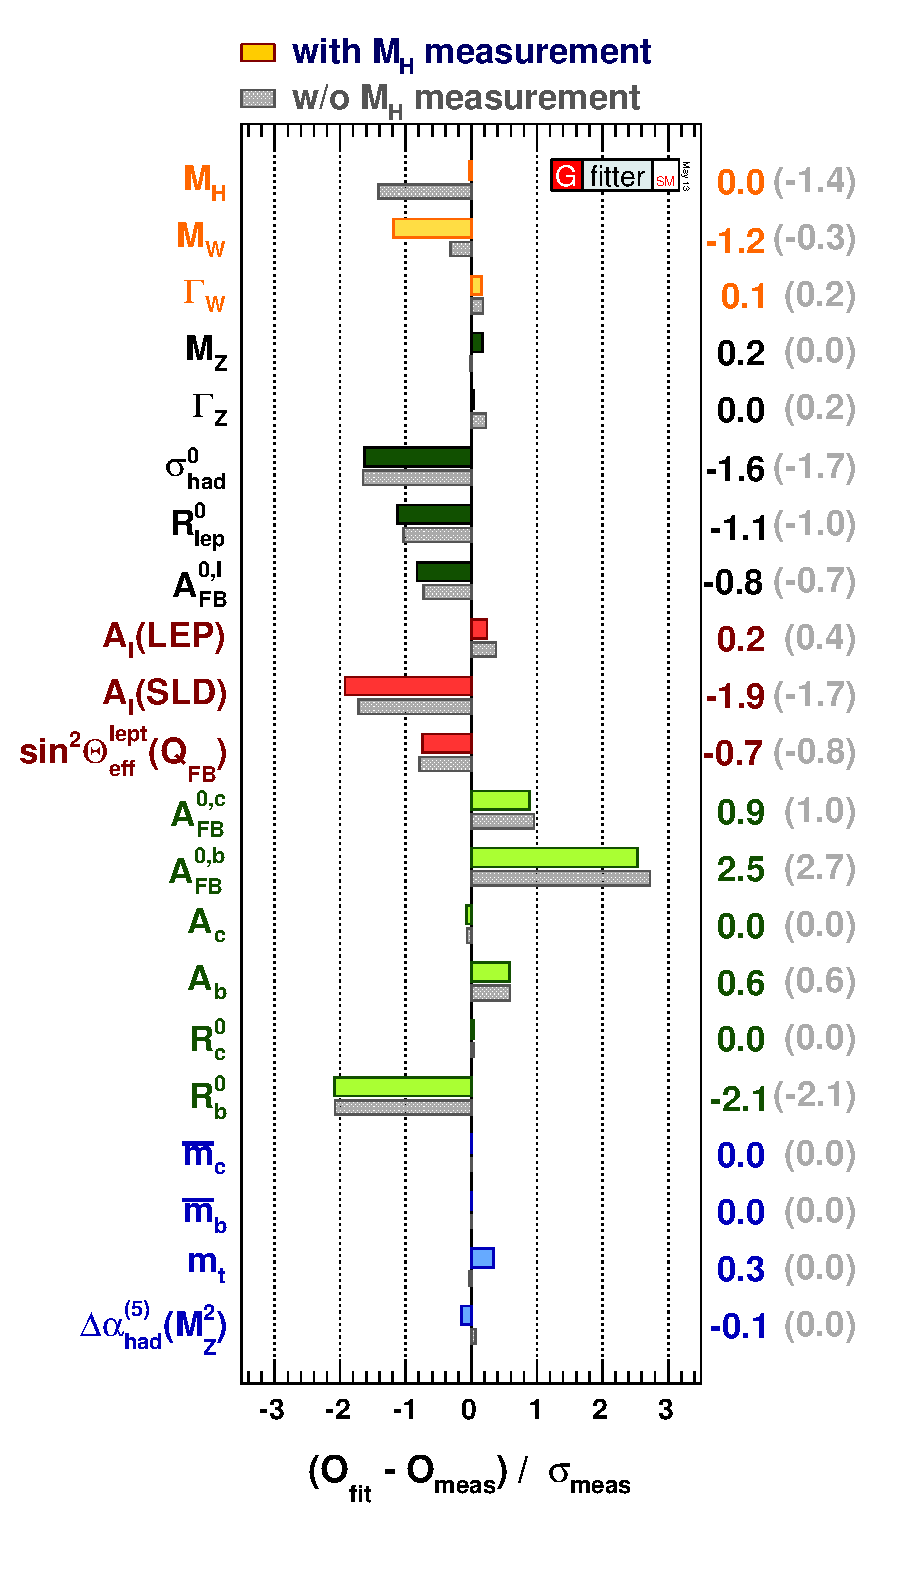
\includegraphics[width=0.7\textwidth]{Theory/Figures/2013_05_29_PullPlotTwoBarsCol_logo.eps}
%  \caption{Gfitter}
%  \label{fig:gfitter_pulls}
%\end{wrapfigure}
\begin{figure}[t!]
  \centering
        \begin{subfigure}{0.39\textwidth}
  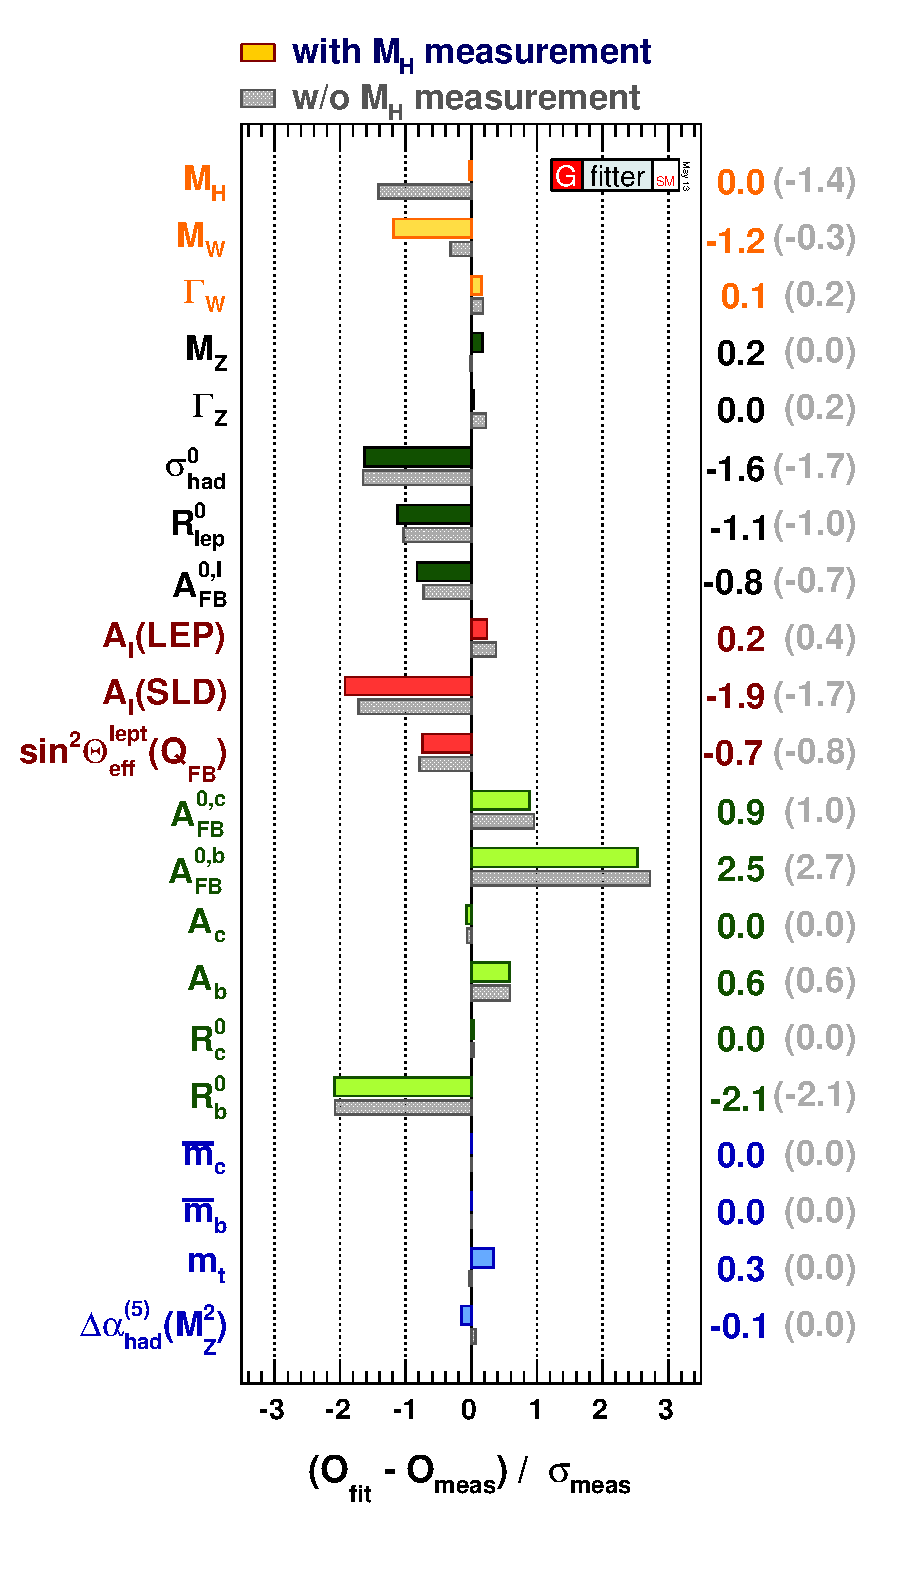
\includegraphics[width=\textwidth]{Theory/Figures/2013_05_29_PullPlotTwoBarsCol_logo.eps}
     \caption{}
  \label{fig:gfitter_pulls}
     \end{subfigure}
     \begin{subfigure}{0.6\textwidth}
    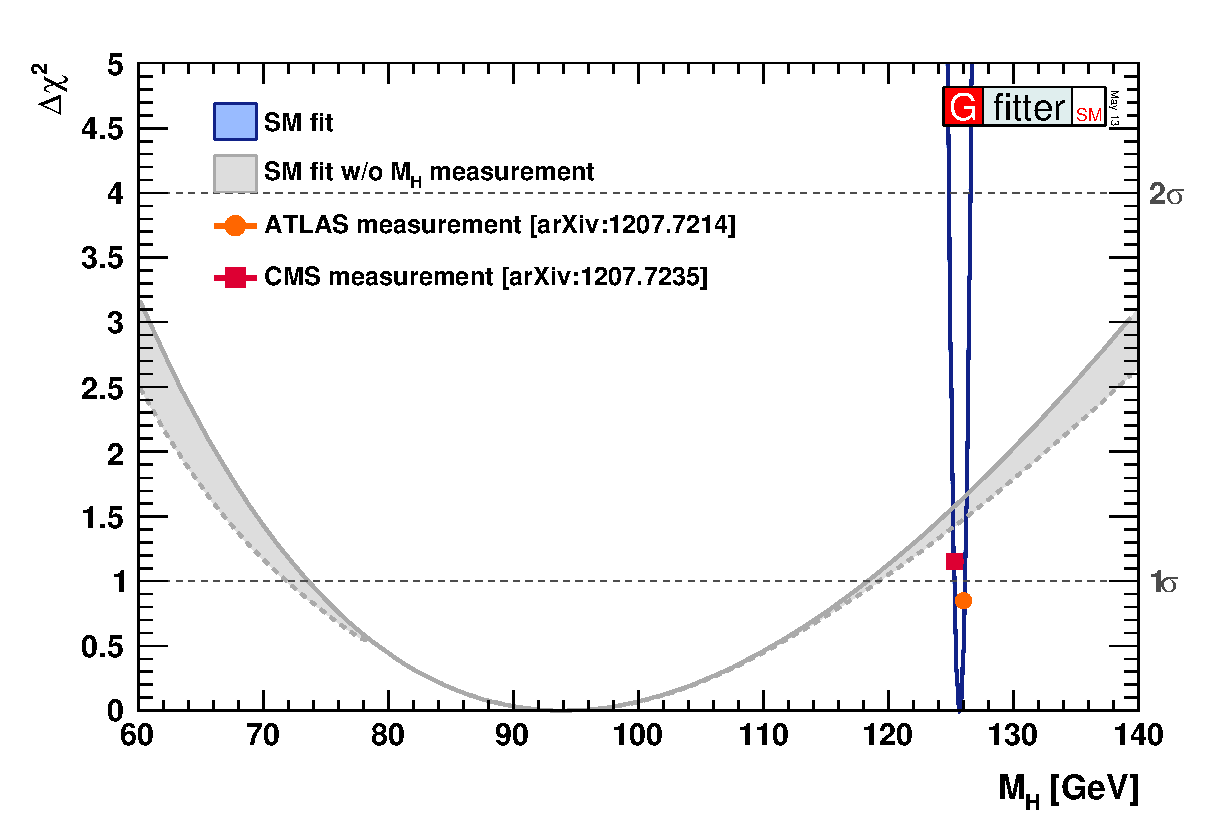
\includegraphics[width=\textwidth]{Theory/Figures/2013_05_29_HiggsScan_logo.eps}
     \caption{}
  \label{fig:gfitter_higgs}
     \end{subfigure}
  \caption{
    Left: pull values for the SM fit with and without inclusion of $M_H$ in the fit. The pull values are defined as deviations between experimental measurements and theoretical calculations in units of the experimental uncertainty.  
    Right: $\Delta \chi^2$ as a function of Higgs boson mass $M_H$, with (blue band) and without the $M_H$ measurements (gray band).
}
  \label{fig:gfitter}
\end{figure}

%\begin{figure}[t!]
%  \centering
%  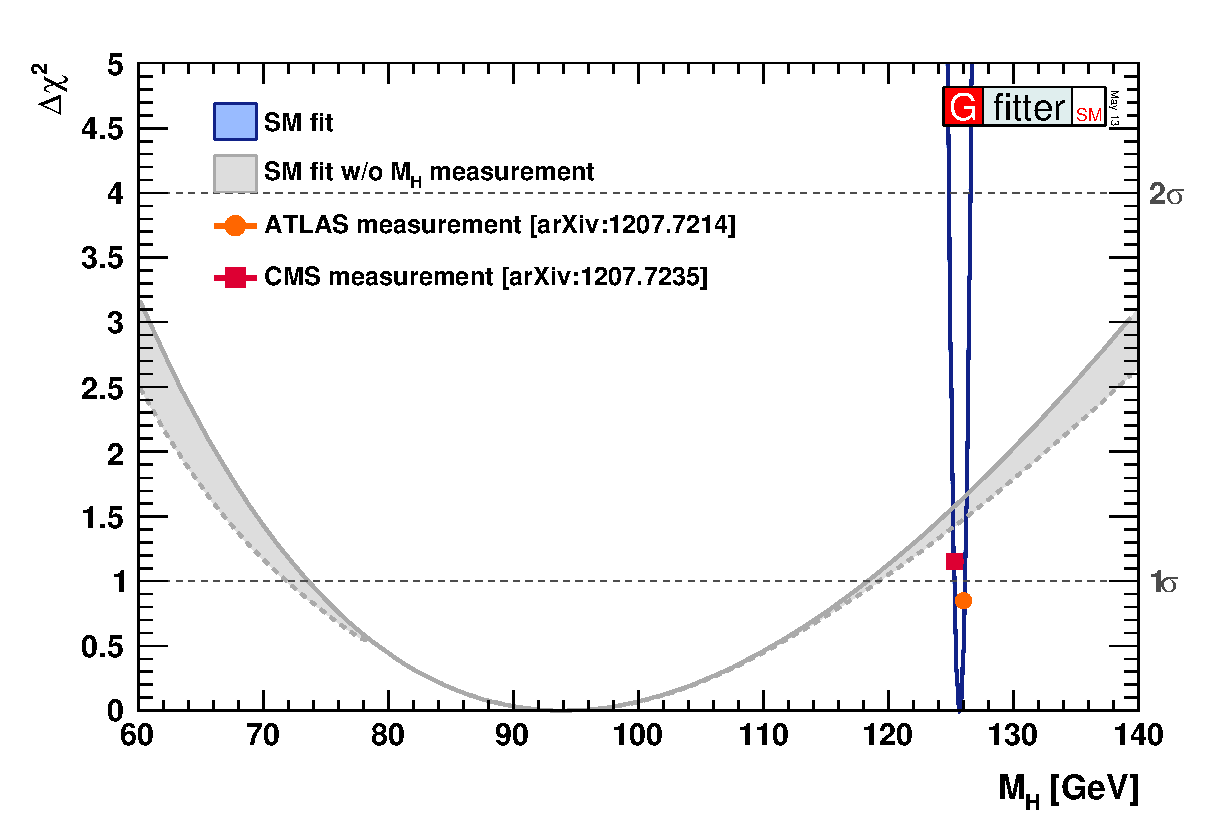
\includegraphics[width=0.7\textwidth]{Theory/Figures/2013_05_29_HiggsScan_logo.eps}
%  \caption{Gfitter}
%  \label{fig:gfitter_higgs}
%\end{figure}

The last missing piece of the SM was found in 2012, when both the ATLAS and CMS collaborations announced the observation of a new particle compatible with the Higgs boson hypothesis~\cite{Aad:2012tfa,Chatrchyan:2012ufa}.
The mass of the new particle was found to be $\unit[\sim 125]{\GeV}$~\cite{Aad:2015zhl}, well within the mass interval allowed by the indirect constraint of the electroweak fit.
Further measurements of the newly discovered particle confirmed that it is a scalar and a positive CP eigenstate~\cite{Aad:2013xqa}.
As of today, the couplings to the rest of the SM particles have been found to be in agreement with those of the SM Higgs boson. 

\subsection{Shortcomings of the Standard Model}
\label{subsec:shortcomings}
Despite the remarkable successes of the SM, there are a number of theoretical and experimental evidences that can not be accommodated into the framework.
This leads to the general conclusion that the SM has to be regarded as an effective theory, the low energy realization of a more complete theory that would be able to explain the whole spectrum of observations. While the detailed formulation of such ``Theory of Everything'' is not yet available, the investigation of the aspects where the SM fails to give a satisfactory answer can shed some light into the details of this more general theory.
\begin{itemize}
  \item One of the few experimental observations that are not explained by the SM are neutrino oscillations~\cite{Fukuda:1998mi}. Although neutrino masses are not measured directly, the measurement of oscillations requires that there is a mass difference between the different neutrino generations. A mass term for neutrinos is not present in the SM, although introducing right-handed neutrinos, or alternatives such as Majorana neutrinos can be accommodated.
  \item Measurements of the rotation curves of galaxies~\cite{Begeman:1991iy} and gravitational lensing led to the inference of the existence of non-luminous matter denominated \textit{dark matter} in the Universe.
    This was also verified in measurements of large-scale structures and cosmic microwave background~\cite{Larson:2010gs,Ade:2013zuv}.
    Dark matter doesn't interact through the electromagnetic force and therefore can not be observed, but its presence is made evident through gravitational effects. The SM has no candidate particle that can account for the large measured fraction of dark matter, encompassing more than \unit[80]{\%} of the total matter in the universe.
  \item %At the moment of the Big Bang, matter and antimmater should have been produced in the same amount, however there is a clear asymmetry and matter remains. 
    The SM can not fully explain the matter/anti-matter asymmetry observed in the Universe. Although CP-violation is described by the presence of a phase in the CKM matrix, the amount of CP-violation is not big enough as to explain the current asymmetry.
  \item The SM has 19 arbitrary parameters, out of them 9 fermion masses. The hierarchical mass structure of the SM fermions, 
    %shown in figure~\ref{fig:particle_masses}
    ranging from $\sim\unit[1]{\mev}$ for the first generation of fermions,\footnote{If neutrino masses are considered, for which the current bounds are $\sim$ eV, this difference increases by six more orders of magnitude. } to about \unit[173]{\gev} of the top quark, is not understood. Also the question of why exactly three families of fermions exist has no justification. 
    The arbitrariety of parameters in the SM, and in particular of the fermion masses, introduces the \textit{naturalness} problem. A ``natural'' theory is characterized by free parameters with values of the same order of magnitude. This does not happen in the SM, where the difference in masses spans five orders of magnitude.
    This is not a problem to the theory itself, but such huge differences in arbitrary parameters are usually considered as unnatural and a possible indication of unknown principles underlying a more complete theory encompassing the SM.
%    \begin{figure}[bh!]
%      \centering
%      \includegraphics[width=0.5\textwidth]{Theory/Figures/particle_masses.png}
%      \caption{Masses}
%      \label{fig:particle_masses}
%    \end{figure}
%    Other shortcomings of the SM are not at the fundamental level but rather unsettling observations that may point to the existence of a theory that extends the SM in order to describe the physics at higher energies. 
  \item A very important missing piece towards a Theory of Everything is the introduction of a quantum field theory for gravity. At energies of the order of the Planck scale, 
    ${M_P = \left(8\pi G_\text{Newton}\right)^{-1/2} = \unit[10^{18}]{\gev}}$, 
      %{$M_P = \left(8\pi G_\text{Newton}\right)^{-1/2} = \unit[2.4\times 10^{18}]{GeV}$}, 
    quantum gravitational effects are not negligible and a new model should replace the SM. In the hypothetical absence of new physics below this scale, the requirement that the SM has to be valid up to the Planck scale introduces a new problem known as the ``hierarchy problem''.
\end{itemize}

\subsubsection{The hierarchy problem} 
A further argument pointing to the need for new theories beyond the SM is the ``hierarchy problem'', which can be defined as the fact that the difference between the weak scale and the Planck scale, $M_P/M_W$, is so huge.
This is not a fundamental problem of the SM itself, but it introduces a disturbing sensitivity of the Higgs potential to new physics in almost any imaginable extension of the SM.
Unlike the fermions and gauge bosons, elementary scalars as the Higgs boson are not protected by chiral or gauge symmetries against large radiative corrections to their masses.
%In particular, in the SM there is no mechanism to prevent scalar particles from acquiring large masses through radiative corrections.
For this reason, the Higgs field receives enormous corrections from the virtual effects of any SM particle it couples to.

\begin{figure}[!t]
  \centering
   \begin{subfigure}{0.49\textwidth}
      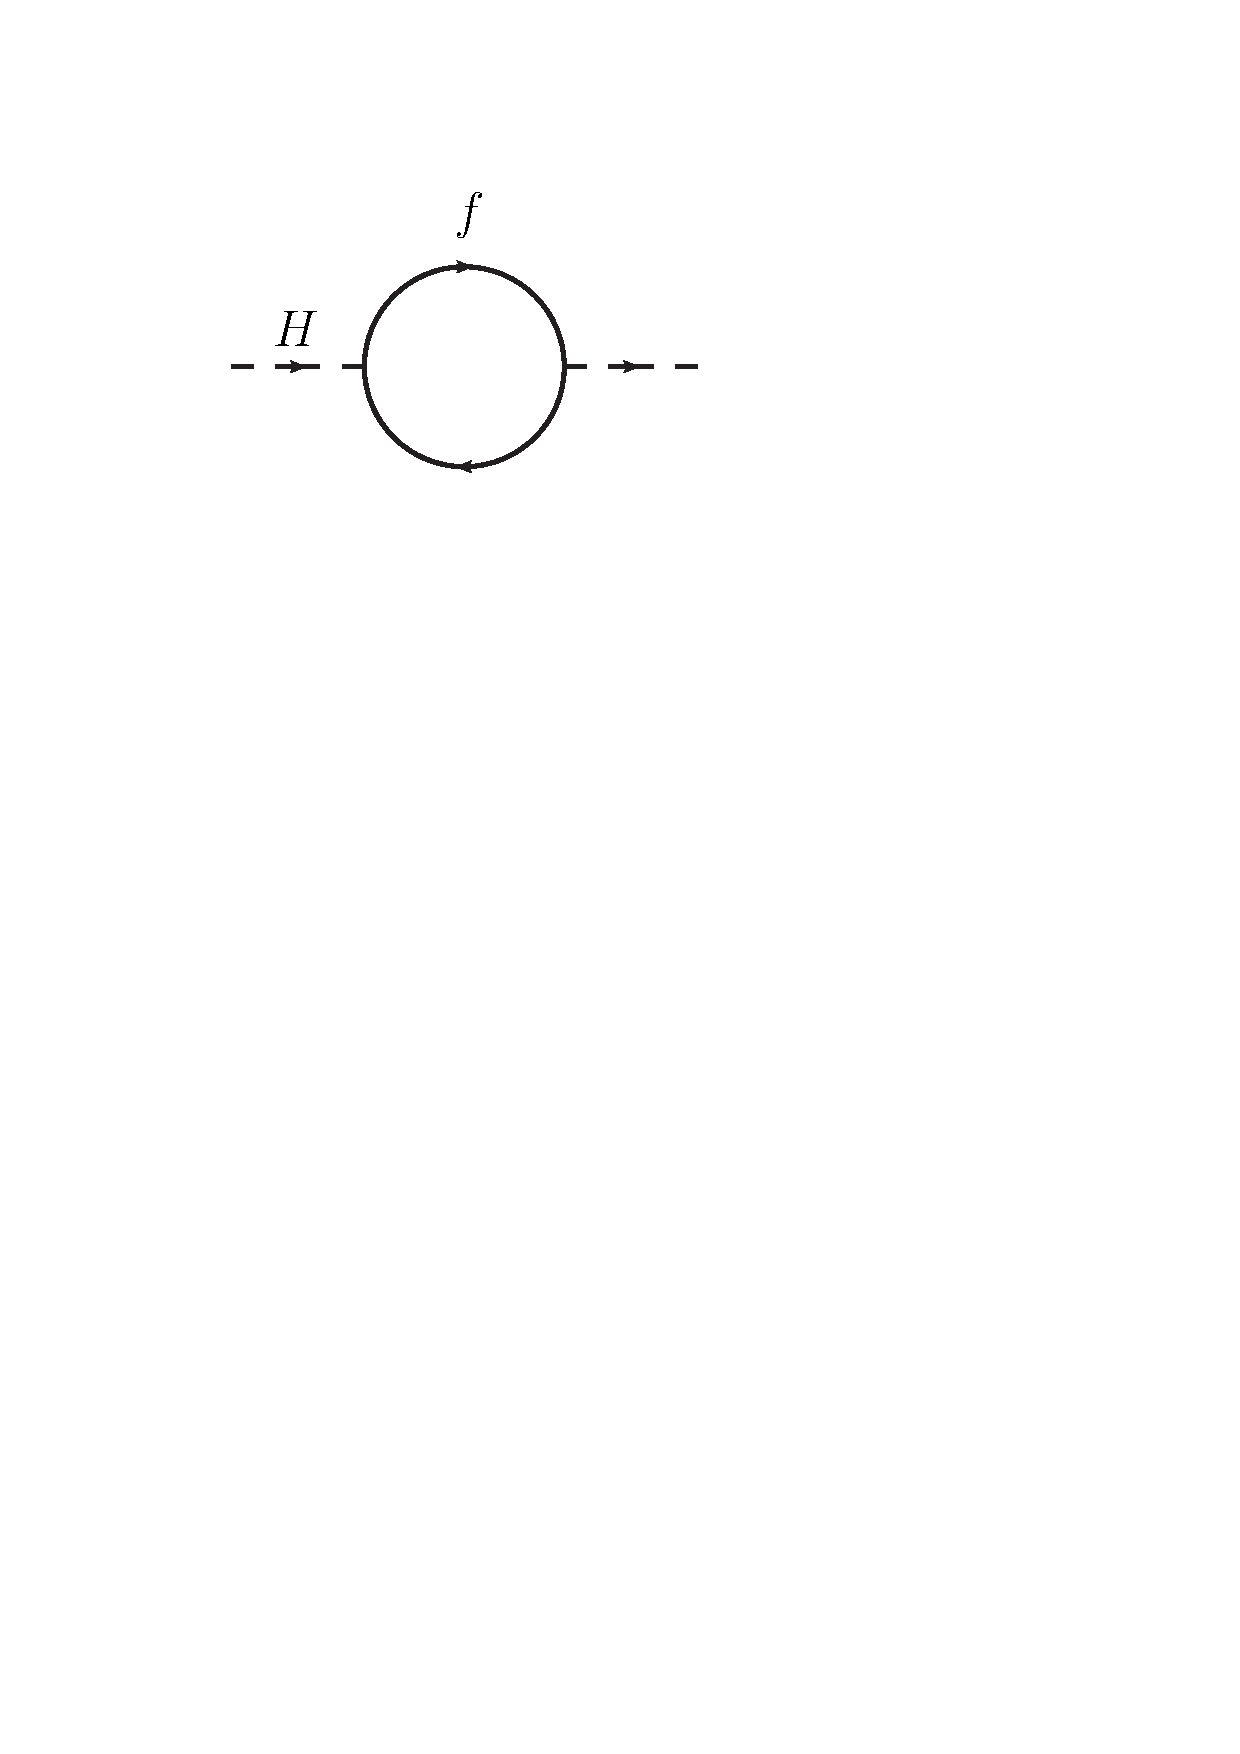
\includegraphics[width=\textwidth]{Theory/FeynmanGraphs/loopFermion.pdf}
     \caption{}
      \label{fig:loopFermion}
 \end{subfigure}
   \begin{subfigure}{0.49\textwidth}
      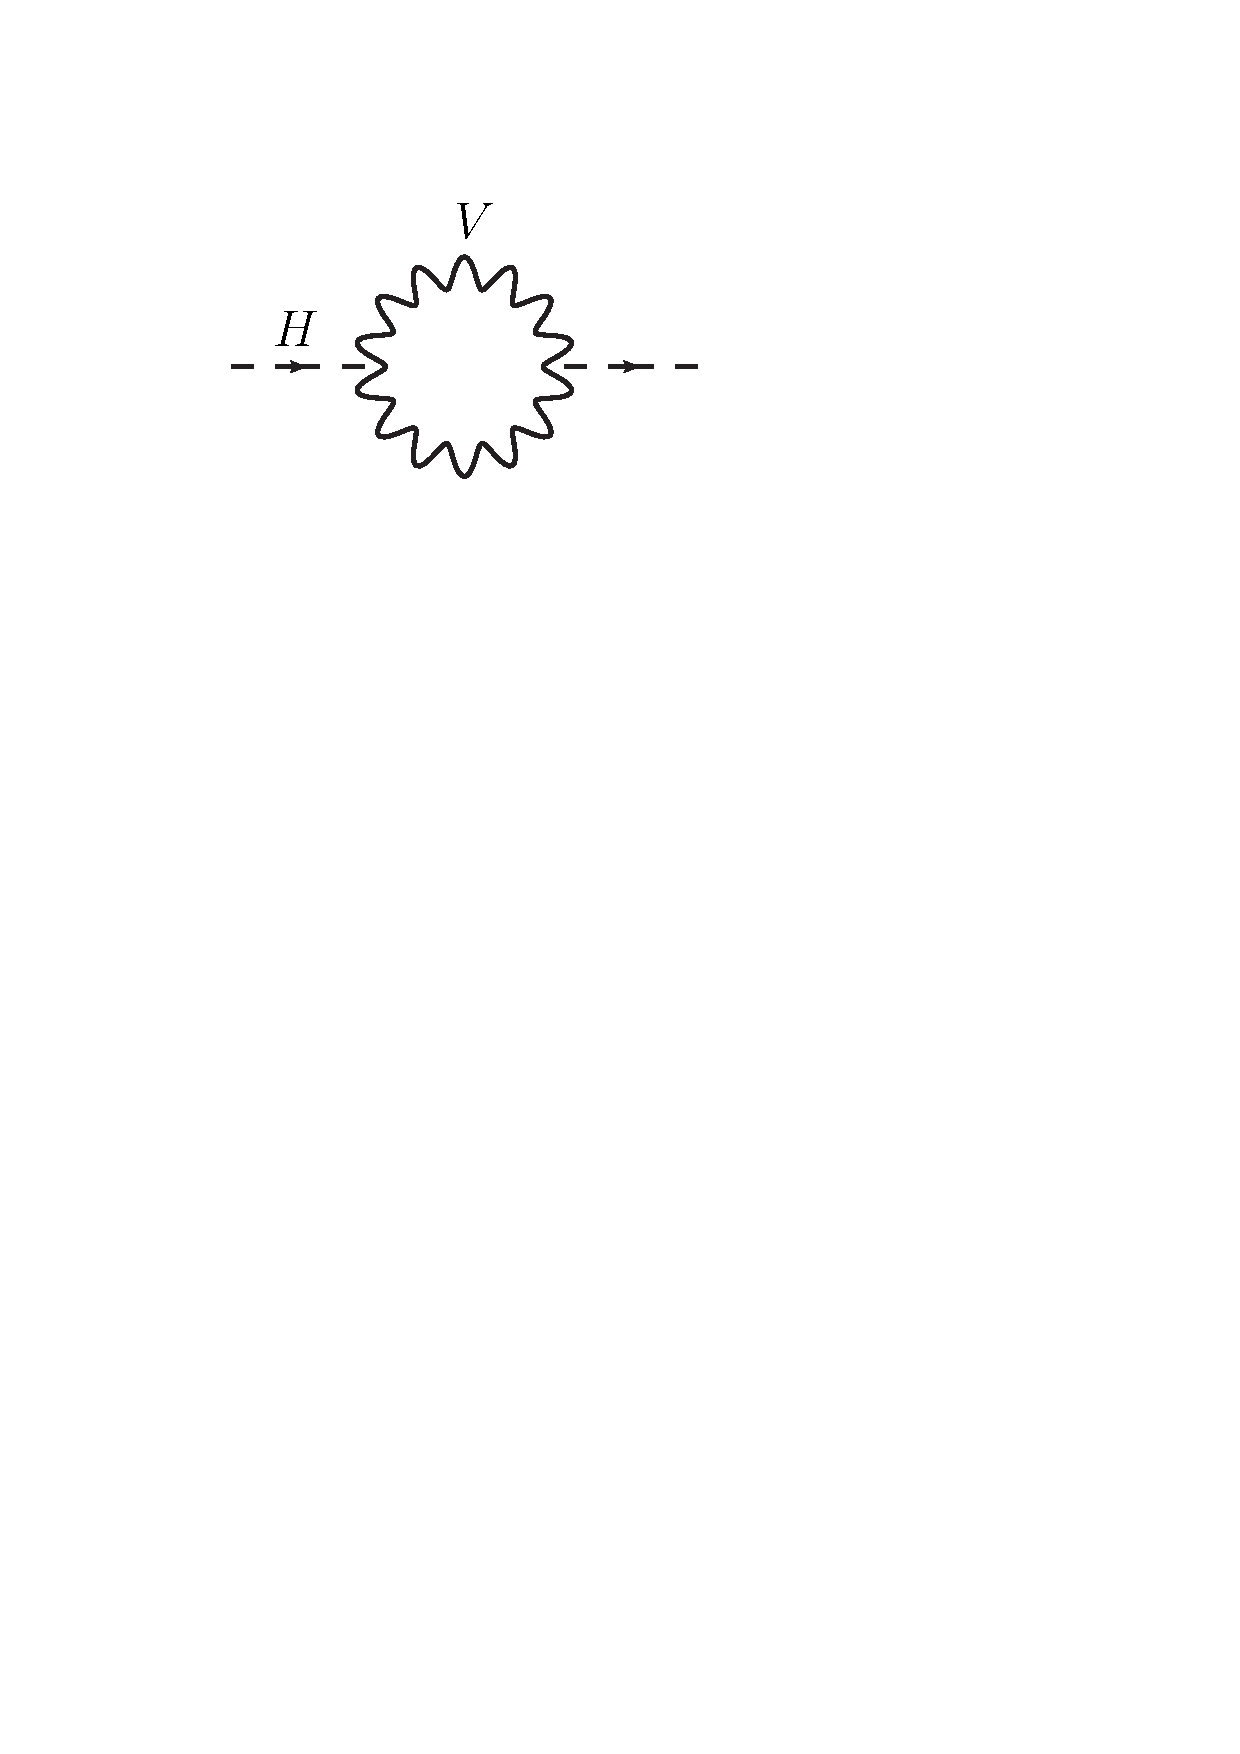
\includegraphics[width=\textwidth]{Theory/FeynmanGraphs/loopBoson.pdf}
     \caption{}
      \label{fig:loopBoson}
 \end{subfigure}
  \caption{Examples of one-loop quantum corrections to the Higgs mass due to fermions (left) and bosons (right).}
%  \label{fig:HiggsLoop}
\end{figure}

Due to these corrections, the Higgs boson mass is:

\begin{equation} 
  m_H^2 = (m_H)_{0}^{2} + \Delta m_H^2~,
  \label{eq:HiggsMassTotal}
\end{equation}

\noindent where $(m_H)_0$ is the bare Higgs mass and $\Delta m_H^2$ is the Higgs mass correction which, for the case of a fermion loop as in figure~\ref{fig:loopFermion}, is given by:

\begin{equation}
  \Delta m_H^2 = -\frac{|y_f|^2}{16\pi^2}\left[2\Lambda^2 + \mathcal{O}\left(m_f^2\ln{\left(\frac{\Lambda}{m_f}\right)}\right)\right]~,
  \label{eq:HiggsMassCorrectionFermion}
\end{equation}

\noindent being $y_f$ the Yukawa coupling of the fermion $f$ and being $\Lambda$ a cutoff.
The latter is interpreted as the energy scale at which new physics enters and the SM ceases to be valid.
Similar corrections arise also from gauge-boson loops, as shown in figure~\ref{fig:loopBoson}.
If the SM needs to describe Nature up to $M_P$, then the quantum corrections to the Higgs mass can be up to 30 orders of magnitude larger than the measured Higgs boson mass squared.
In order to recover the measured mass of the Higgs boson, the value of the bare Higgs mass and the corrections have to exactly cancel to an incredible precision. This precise cancellation is known as \emph{fine tuning}.

Since this cancellation over 16 orders of magnitude, although not forbidden, seems to be a too lucky coincidence, several extensions of the SM have been proposed where different mechanisms are present to keep the Higgs boson mass at the electroweak scale.

%\subsubsection{The top Yukawa coupling}
The largest correction to the Higgs boson mass comes from the top quark, since it is the heaviest particle in the SM. The latest Tevatron--LHC combination for the top mass yields: $m_{\mathrm{t}}=173.34 \pm 0.76 \GeV$~\cite{ATLAS:2014wva}.
This value implies that the top quark is the only particle in the SM to have a Yukawa coupling $y_{\mathrm{t}}$ very close to unity:
\begin{equation}
  y_{\mathrm{t}} = \frac{\sqrt{2}m_{\mathrm{t}}}{v} = 0.996 \pm 0.005~.
  \label{eq:top_yukawa}
\end{equation}
%It is also the particle that induces the largest radiative correction to the top mass.
While in the SM $y_{\mathrm{t}}$ is one of the free parameters of the theory, 
such particular value suggests that the top quark might have a special role in the electroweak symmetry breaking mechanism and the mass hierarchy pattern.
%At the same time, several proposed extensions of the SM predict the presence of new particles strongly coupling to the top quark.

\section{Beyond the Standard Model}
\label{sec:BSM}
Over the years, many theories have been proposed that try to extend the SM in order to solve one or several of its shortcomings. Several of these theories provide solutions for the hierarchy problem. In the following, some of these scenarios are reviewed, highlighting the phenomenology of those models predicting \ttbar\ final states with additional heavy-flavor jets, which is the signature explored in this dissertation.
\subsection{Supersymmetry}
The hierarchy problem can be solved if for each SM particle a new particle is introduced with spin differing by 1/2, that also couples to the Higgs boson. In the example of a SM fermion, a new boson $S$ is introduced, and the correction to the Higgs mass is given by:
\begin{equation}
  \Delta m_H^2 = \frac{y_S^2}{16\pi^2}\left[2\Lambda^2 + \mathcal{O}\left(m_S^2\ln{\left(\frac{\Lambda}{m_S}\right)}\right)\right],
  \label{eq:HiggsMassCorrectionScalar}
\end{equation}
where it has to be highlighted that this correction has opposite sign to the fermion contribution in equation~\ref{eq:HiggsMassCorrectionFermion}. If $y_S = |y_f|$, all the fermion terms have a counter term that naturally cancels the quadratic divergence introduced. The residual correction terms to the Higgs mass, ignoring the logarithmic contributions, would be:

\begin{equation}
  \Delta m_H^2 = \frac{y_f^2}{16\pi^2} |m_S^2 - m_f^2|~.
  \label{eq:HiggsMassCorrectionNoQuadratic}
\end{equation}

Invoking ``naturalness'' arguments, the size of the corrections is expected to be smaller than $m_{H}$, which leads to:

\begin{equation}
  |m_S^2 - m_f^2| \lesssim \unit[1]{TeV}^2~.
  \label{eq:HiggsNaturalnessCondition}
\end{equation}

This can be understood as the range of validity of the SM: at the \tev\ scale superpartners of the SM particles can be produced and the SM is replaced by its supersymmetric extension. This scale, derived from naturalness arguments, is not a strict upper bound on supersymmetric extensions, but rather a desirable scale where supersymmetry could stabilize the corrections to the Higgs mass before developing its own hierarchy problem, as discussed below.

The postulation of new particles canceling to first order all SM corrections to the Higgs mass is done through the introduction a new symmetry: supersymmetry.
In fact, supersymmetry (SUSY) seems to be the last possible extension of the Lorentz group~\cite{Haag:1974qh}.
A supersymmetry transformation turns a bosonic state into a fermionic state and viceversa~\cite{Drees:1996ca}. 
%The SM particles can then be organized into supermultiplets with their supersymmetric partners
The mass of the superpartners is predicted to be the same as the SM particles but, since no supersymmetric particle has been observed yet, supersymmetry must be a broken symmetry and supersymmetric particles' masses have to be above the reach of current experiments.

The extension of the SM through a supersymmetry is not unique: the number of generators in the symmetry group, as well as the composition and arrangement of the SM particles into supermultiplets allow many possibilities. Supersymmetry is not a fixed model but a framework from which many SM extensions can be derived. 

The minimal supersymmetric Standard Model (MSSM) is a model that introduces the minimal amount of new particles. It consists of one single operator in the symmetry group and every SM particle is paired with one single superpartner. Partners of the fermions are denoted with the prefix ``s'', for example the superpartner of the top quark is referred to as \textit{stop}, and partners of the SM bosons are labeled with the suffix ``ino''. The Higgs sector requires the introduction of an additional complex doublet, therefore producing five particles after giving mass to the SM bosons. Table~\ref{tab:MSSM_content} shows the arrangement and notation of the MSSM particle content.

\begin{table}[!ht]
  \begin{center}
    \begin{small}
      %\setlength{\tabcolsep}{0.0pc}
      %\begin{tabular*}{\textwidth}{@{\extracolsep{\fill}}ccccc}
      \begin{tabular}{ccccc}
        \toprule
        \toprule
        \textbf{Names} & \textbf{Spin} & \textbf{$P_R$} & \textbf{Gauge eigenstates}      & \textbf{Mass Eigenstates} \\
        \midrule
        Higgs bosons   & $0$           & $+1$                 & $H_u^0$ $H_d^0$ $H_u^+$ $H_d^-$ & $h^0$ $H^0$ $A^0$ $H^\pm$ \\
        \midrule
        \multirow{3}{*}{Squarks} & \multirow{3}{*}{$0$} & \multirow{3}{*}{$-1$} & $\tilde{u}_L$ $\tilde{u}_R$ $\tilde{d}_L$ $\tilde{d}_R$ & same \\
        &                      &                       & $\tilde{s}_L$ $\tilde{s}_R$ $\tilde{c}_L$ $\tilde{c}_R$ & same \\
        &                      &                       & $\tilde{t}_L$ $\tilde{t}_R$ $\tilde{b}_L$ $\tilde{b}_R$ & $\tilde{t}_1$ $\tilde{t}_2$ $\tilde{b}_1$ $\tilde{b}_2$ \\
        \midrule
        \multirow{3}{*}{Sleptons}& \multirow{3}{*}{$0$} & \multirow{3}{*}{$-1$} & $\tilde{e}_L$ $\tilde{e}_R$ $\tilde{\nu}_e$ & same \\
        &                      &                       & $\tilde{\mu}_L$ $\tilde{\mu}_R$ $\tilde{\nu}_\mu$ & same \\
        &                      &                       & $\tilde{\tau}_L$ $\tilde{\tau}_R$ $\tilde{\nu}_\tau$& $\tilde{\tau}_1$ $\tilde{\tau}_2$ $\tilde{\nu}_\tau$ \\
        \midrule
        Neutralinos    & $1/2$           & $-1$                 & $\tilde{B}^0$ $\tilde{W}^0$ $\tilde{H}_u^0$ $\tilde{H}_d^0$ & $\ninoone$ $\ninotwo$ $\ninothree$ $\ninofour$ \\
        \midrule
        Charginos      & $1/2$           & $-1$                 & $\tilde{W}^\pm$ $\tilde{H}_u^+$ $\tilde{H}_d^-$ & $\chinoonepm$ $\chinotwopm$ \\
        \midrule
        Gluino         & $1/2$           & $-1$                 & $\gluino$ & same \\
        \bottomrule
        \bottomrule
      \end{tabular}
    \end{small}
  \end{center}
  \caption[Predicted MSSM spectra.]{The predicted particle spectra in the MSSM (sfermion mixing for the first two families is assumed to be negligible).}
  \label{tab:MSSM_content}
\end{table}

The most general MSSM can contain operators that violate baryon and/or lepton number, thus allowing proton decays. The non-observation of proton decays forbids the existence of such terms.\footnote{
Strictly speaking, it imposes very stringent upper limits on the coefficients of those operators.}
A possibility to avoid these operators is to introduce a new discrete symmetry named $R$-parity. The conserved quantum number is defined as:

\begin{equation}
  P_R = (-1)^{3(B-L)+2s}~,
  \label{eq:RparityDefinition}
\end{equation}

\noindent where $B$ and $L$ refer to the baryon and lepton quantum numbers respectively and $s$ is the spin of the particle.
This definition sets all the SM particles to have $P_R = +1$ while the SUSY partners have $P_R = -1$.

\subsubsection{Supersymmetry phenomenology}
The conservation of the $R$-parity has several phenomenological consequences:

\begin{itemize}
  \item It prevents baryon and lepton quantum numbers to be violated, therefore removing terms that allow proton decay.
  \item There can be no mixing between the SM particles and their supersymmetric partners.
  \item SUSY particles can only be produced in pairs in the collisions of SM particles.
  \item The lightest SUSY particle (LSP) is stable, and therefore constitutes a good candidate for dark matter if electrically neutral.
\end{itemize}

After electroweak symmetry breaking, the supersymmetric partners mix giving rise to the mass eigenstates. 
The neutral higgsinos ($\tilde{H}_u^0$ and $\tilde{H}_d^0$) and the neutral gauginos ($\tilde{B}$ and $\tilde{W}^0$) combine to form four mass eigenstates named neutralinos.
The charged higgsinos ($\tilde{H}^+_u$ and $\tilde{H}^-_d$) and the winos ($\tilde{W}^+$ and $\tilde{W}^-$) mix to form two mass eigenstates with electric charge~$\pm 1$, named charginos.

In the sfermion sector, mixing across generations can cause large contributions to flavor changing neutral current processes~\cite{Ellis:1981ts} and is usually removed. However, mixing between the left-handed and the right-handed sfermions\footnote{
  The ``handedness'' of the scalar superpartners does not refer to their helicity, but to that of their SM partners.
}
of the same generation depends on the mass of the SM fermion, and therefore can't be neglected for the third generation superpartners.
After mixing, the mass eigenstates are labeled as $\tilde{q}_1$, $\tilde{q}_2$.

The MSSM, with the requirement of R-parity conservation, provides a solution to the hierarchy problem and contains a good candidate for dark matter. However, it also introduces 105 new parameters, to be added to the 19 parameters of the SM.
In order to reduce the number of parameters to be considered, several simplifications and assumptions are introduced in collider searches. Usually, only the sparticles that contribute to a particular final state are considered. The rest of the superpartners are considered heavy enough so that they can be completely decoupled. 
%For the analysis presented in this dissertation, only the top quark partners and the lightest neutralino, \stopone, \stoptwo, \neutralino, are considered to be kinematically accessible at the LHC.

\subsection{Extra dimensions}
The formulation of the SM assumes that our universe exists in a four-dimensional space-time. However, some theories propose that our universe is a four-dimensional ``brane'' embedded in a higher-dimensional space, referred to as ``bulk''. The effect of gravity is therefore diluted in the extra dimensions, giving an explanation for the apparent weakness of the gravitational force.
A general feature of models with extra dimensions is that particles propagating in the extra dimensions manifest in our four-dimensional brane as Kaluza-Klein (KK) states. These are a series of infinite modes, also referred to as ``towers'', where the mass of each Kaluza-Klein mode corresponds to the modulus of its momentum in the direction transverse to the four-dimensional brane.

\subsubsection{Large extra dimensions, ADD model}
In the Arkani-Hamed-Dimopoulos-Dvali (ADD) model~\cite{ArkaniHamed:1998rs}, the only particle that can propagate through the extra dimensions is the graviton, the hypothetical boson of gravity. The extra spatial dimensions are compactified with a radius $R$, on a scale which is small enough as to not have been probed yet. 
The ``effective'' four-dimensional Planck scale is equivalent to $M_P^2 \sim M_D^{2+n} R^n$, where $M_D$ is the fundamental Planck scale in $4+n$ dimensions, where $n$ is the number of extra spatial dimensions. In the ADD model, the electroweak scale $M_{EW}$ is the only fundamental short scale in nature. The equivalence $M_D \sim M_{EW}$ can be obtained for example if $n=2$ and $R \sim \unit[100]{\mu m}$.

Experimentally, the limits on the $M_D$ scale for ADD models are in the range of $\unit[3-5]{\tev}$ for $2-6$ extra dimensions~\cite{Aad:2015zva}, pushing $M_D$ away from the electroweak scale. 

\subsubsection{Universal extra dimensions}
\label{subsubsec:UED}
Other models postulate universal extra dimensions (UED)~\cite{Appelquist:2000nn}, where all SM particles can propagate in the extra dimensions. The main challenge for these theories is recovering the SM behavior after compactification of the extra dimensions. One of the options is the existence of two extra dimensions, which are compactified under the real projective plane geometry (RPP)~\cite{Burdman:2006gy,Cacciapaglia:2009pa}.

A distinctive feature of models with UED is
that each KK vector mode is accompanied by a \mbox{spin-0} particle
in the adjoint representation of the corresponding
gauge group. The partner of the gluon is a massive coloured scalar that is generically referred to as sgluon.

\subsubsection{Randall-Sundrum extra dimensions}
Another particularly interesting model is the Randall-Sundrum (RS) theory~\cite{Randall:1999vf,Contino:2006nn}. Models with extra dimensions usually rely on a factorizable geometry, namely the metric of the four familiar dimensions is independent of the coordinate in the extra dimensions. In the RS theory this assumption is dropped. The universe is considered a five-dimensional anti-de Sitter space ($\text{AdS}_5$) described by a warped geometry and the background metric solves the hierarchy problem~\cite{Randall:1999ee}. 
The background metric contains a multiplicative factor that depends exponentially on the distance to the ``gravity-brane''. The 15 orders of magnitude between the weak and the Planck scale could be explained by the distance from our brane to the gravity-brane.

\subsection{Compositeness}
Throughout the history of physics, several times a particle that was believed elementary revealed its composite nature when studied at higher energy scales. Pions, protons and even atoms were considered elementary at some point. Several new theories propose a similar situation for the SM, where particles that we consider elementary are made of yet unknown constituents which are strongly coupled through new heavy resonances.

Models of partial compositeness are also possible, where elementary and composite particles mix, and the SM particles are in fact linear combinations of elementary and composite states.

\subsubsection{Higgs boson compositeness}
The idea of a composite Higgs boson has its origin in the QCD sector where the pion mass is naturally low. In a theory with spontaneous symmetry breaking, Goldstone bosons arise as scalar, massless particles~\cite{PhysRev.127.965}. If the symmetry is not exact, and is both spontaneously and explicitly broken, then the Goldstone bosons can acquire mass. In this case the boson is called a pseudo-Goldstone boson (PGB). 
%A nice example of a pseudo-Goldstone boson is the pion, which was considered the responsible for quark masses. 
In QCD the flavor chiral symmetry of the Lagrangian is broken spontaneously, generating three massless scalar bosons. The further explicit symmetry breaking operated by the quark masses gives mass also to the pseudo-Goldstone bosons which is, however, much smaller than the other mesons' masses. The three pseudo-Goldstone bosons are the $\pi^{\pm}$ and $\pi^0$ particles, which are not elementary but composed of a quark-antiquark pair.

In a similar way, some theories propose a mechanism of strong electroweak symmetry breaking~\cite{Kaplan1984187}. A new sector is added to the SM containing the Higgs field and new strongly-interacting particles, usually named the composite sector. In the composite sector a global symmetry is spontaneously broken and then, thanks to a small mixing with the SM sector, it is also explicitly broken producing a pseudo-Goldstone boson, the Higgs boson, which is much lighter than the scale of the new sector.
In this scenario the radiative corrections to the Higgs mass don't have to reach the Planck scale since it will reveal its composite nature at the energy scale of the new strong sector.

Strongly interacting theories have usually difficulties to pass electroweak precision tests, or even to compute their contributions. Another problem of these models is explaining the origin of fermion masses.
In the past years, models of pseudo-Goldstone Higgs in the framework of a five-dimensional $\text{AdS}_5$ theory~\cite{ED1,Agashe:2004rs}
 have received increasing attention since the theory is weakly coupled, making it possible to perform calculations, and it can satisfy the bounds from electroweak data.

\subsubsection{Top quark compositeness}
Certain models propose that the top quark is not an elementary particle, but rather a composite or condensate state.
In models with composite particles due to a new strong sector, SM particles can get their masses by mixing with composite states. Given the large mass of the top quark it would be natural to expect the top quark to have a sizable admixture of the composite state and therefore to show properties of compositeness~\cite{Pomarol:2008bh,Kumar:2009vs}. Electroweak precision data strongly constrains the possibility of a composite left-handed top. Therefore, most models focus on right-handed composite top quarks~\cite{Lillie:2007hd,Georgi:1994ha}.

\section{Signatures of BSM theories}
The new particles predicted by the different theories are generally short-lived, and they can be detected by looking for their decay products. 
The analyses discussed in this dissertation explore a final state compatible with the production of a top quark pair with additional heavy-flavor jets. The different theories discussed in section~\ref{sec:BSM} can produce the targeted final state, and their phenomenology is described in the following.

\subsection{Fermionic top partners: vector-like quarks}
Several models predict the existence of vector-like quarks (VLQ), defined as color-triplet \mbox{spin-1/2} fermions whose left- and right-handed chiral components have the same transformation properties under the weak-isospin gauge group~\cite{delAguila:1982fs,AguilarSaavedra:2009es}. 
Vector-like quarks are required if the Higgs  boson is a pseudo-Goldstone boson, they also arise as KK excitations of SM quarks propagating in the bulk and in grand unified theories based on the $E_6$ group~\cite{Frampton:1999xi,Hewett1989193}.
The introduction of vector-like quarks also stabilizes the Higgs boson mass since the quadratic divergences cancel and only a logarithmic divergence remains. The one-loop contributions to the Higgs boson mass are shown in figure~\ref{fig:VLQ_loop}.

\begin{figure}[tb]
  \begin{center}
   \begin{subfigure}{0.32\textwidth}
  	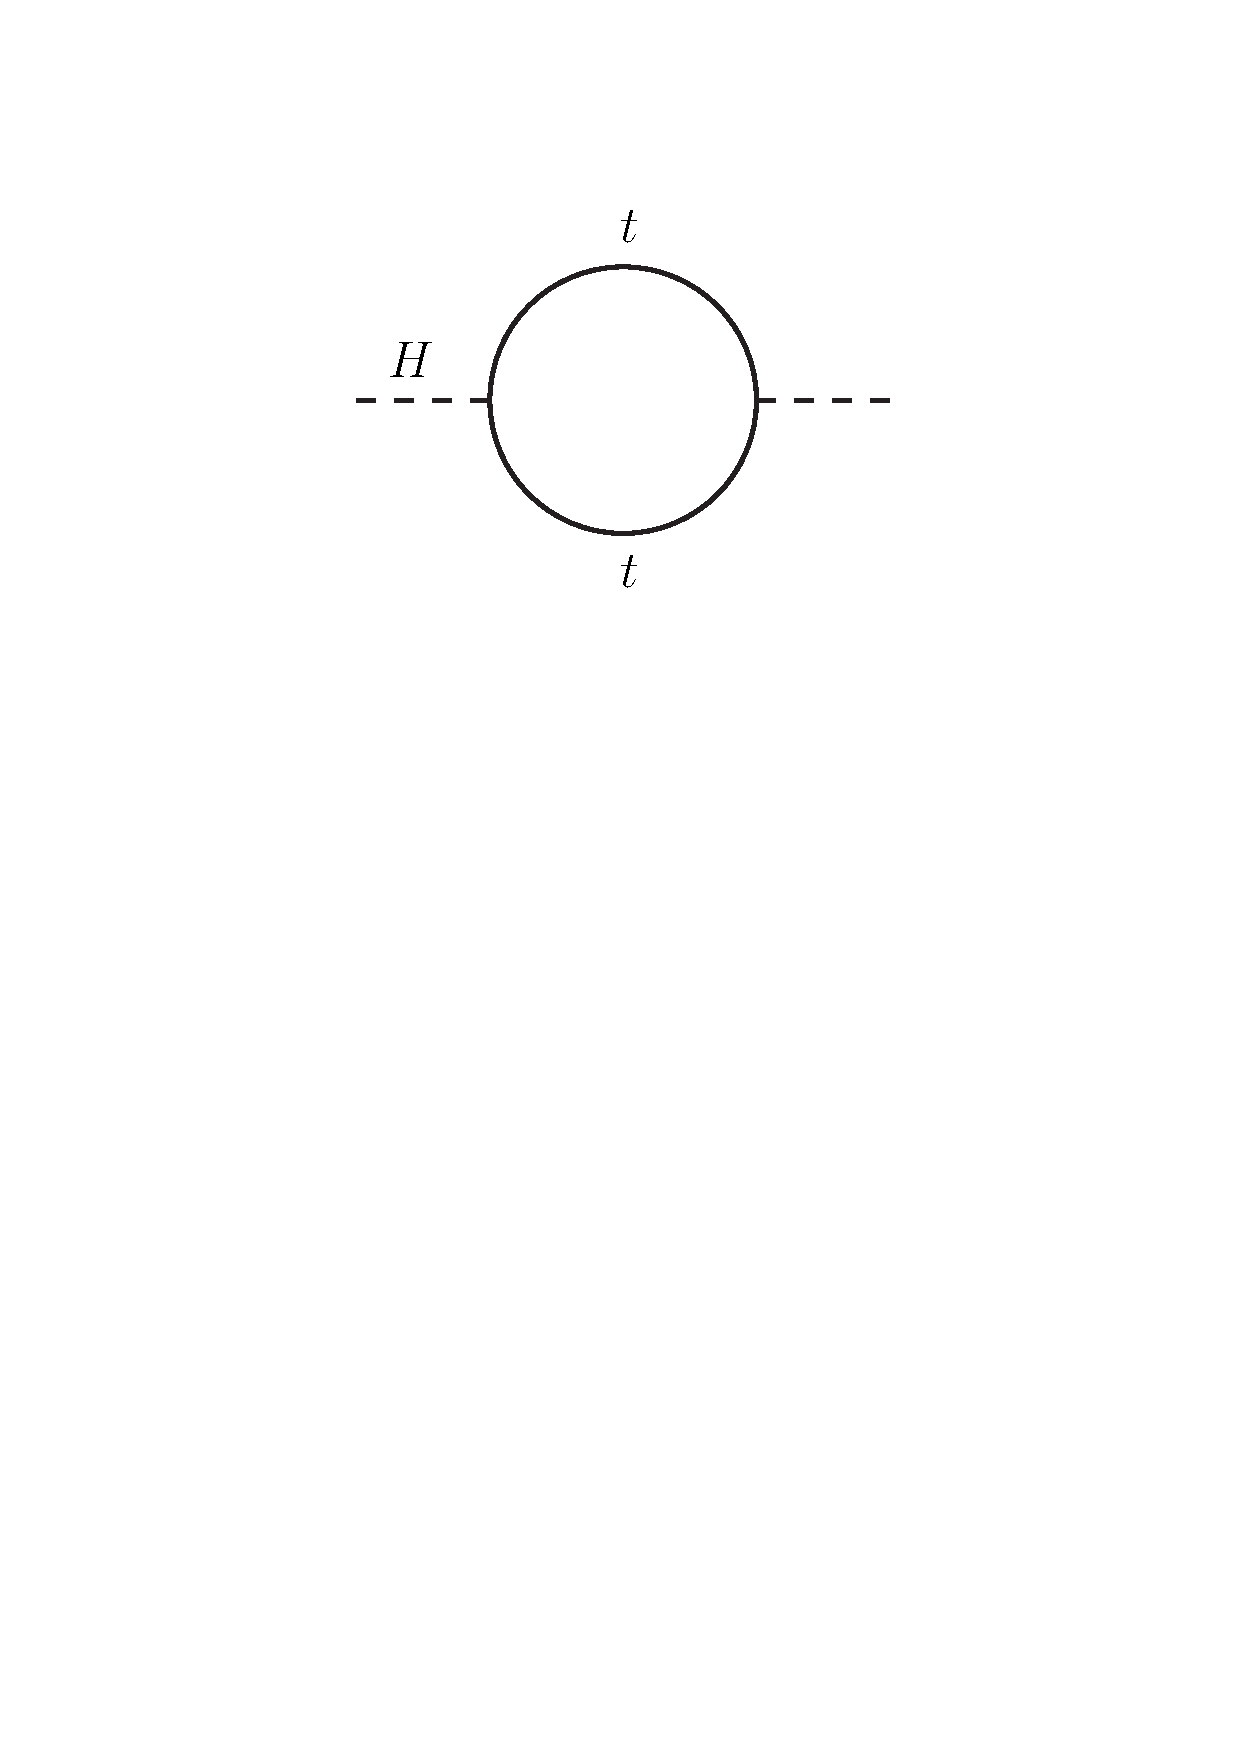
\includegraphics[width=0.92\textwidth]{Theory/FeynmanGraphs/loop_toptop_good}
    \caption{} \end{subfigure}
   \begin{subfigure}{0.32\textwidth}
  	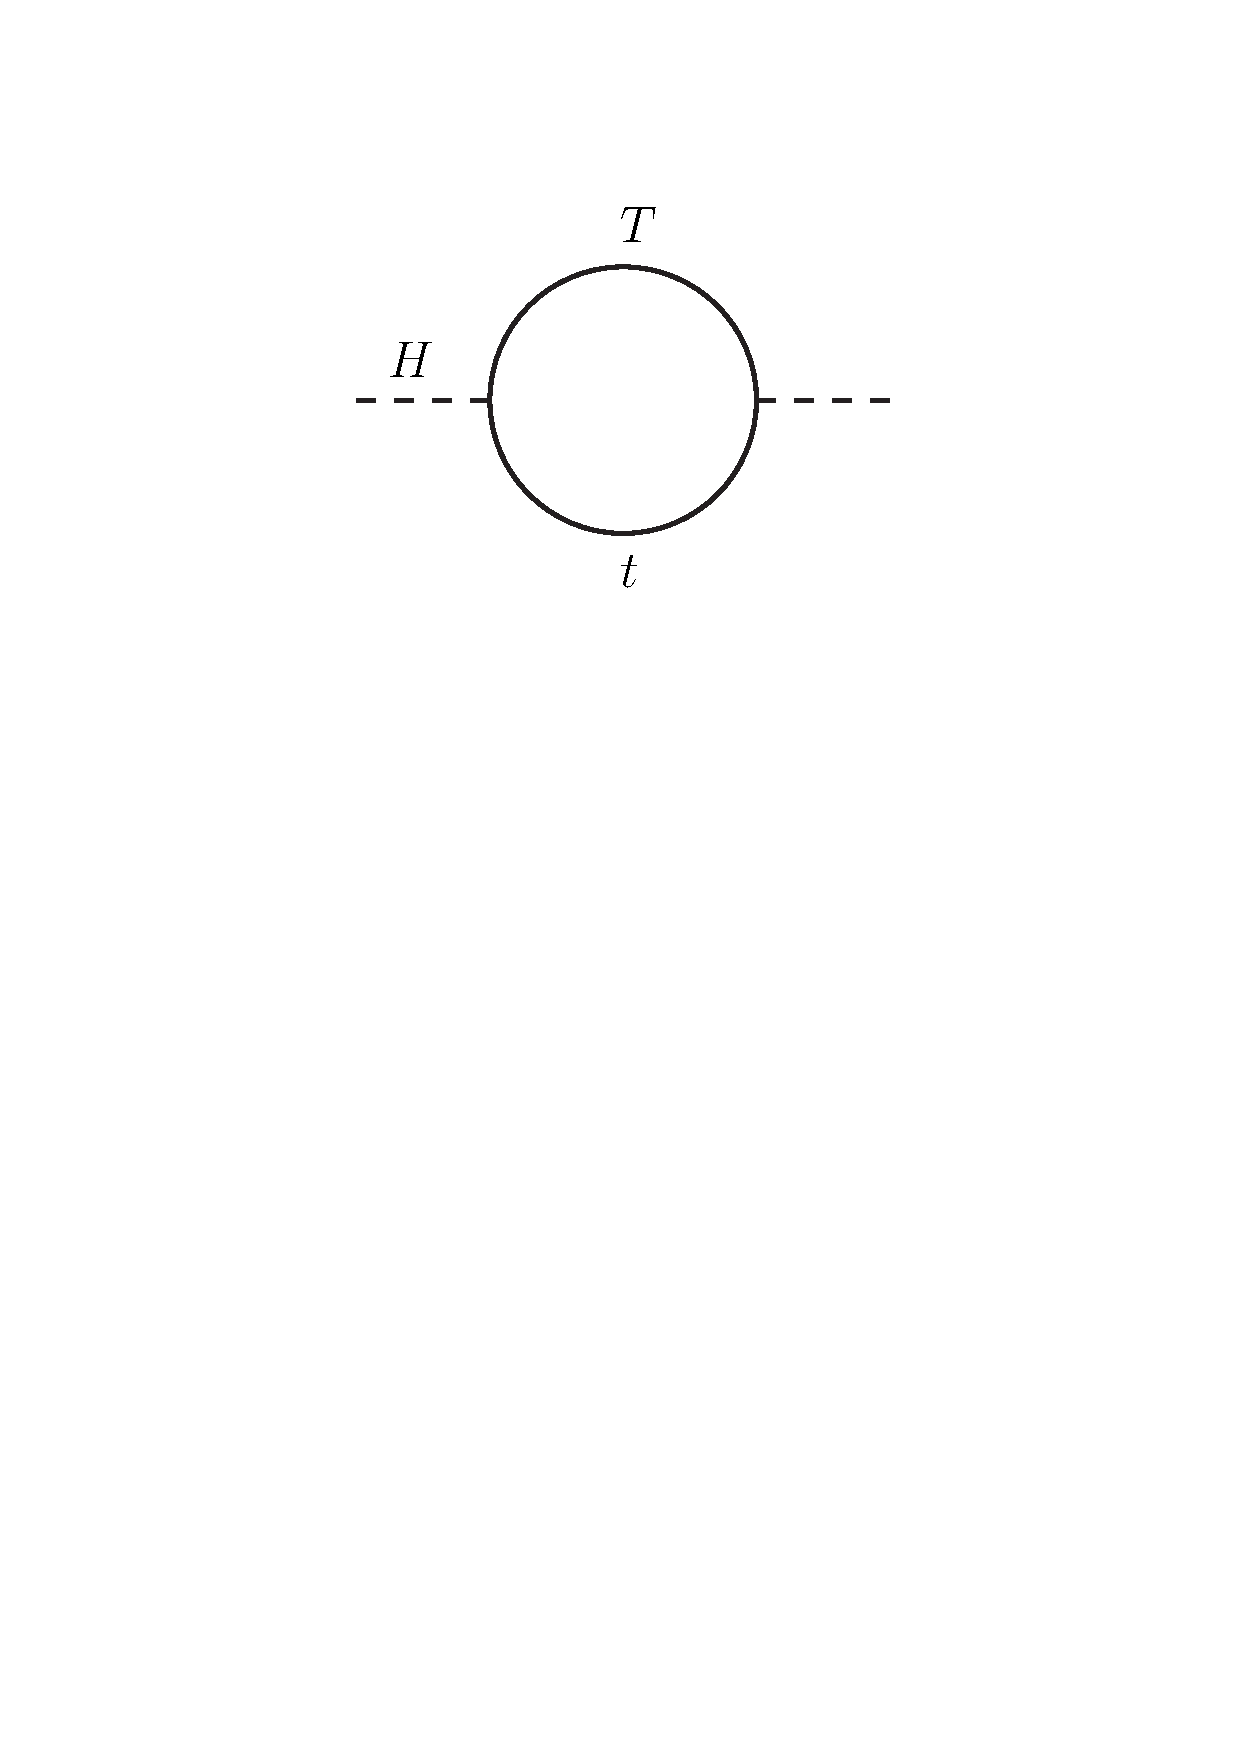
\includegraphics[width=0.92\textwidth]{Theory/FeynmanGraphs/loop_topT_good}
    \caption{} \end{subfigure}
   \begin{subfigure}{0.32\textwidth}
  	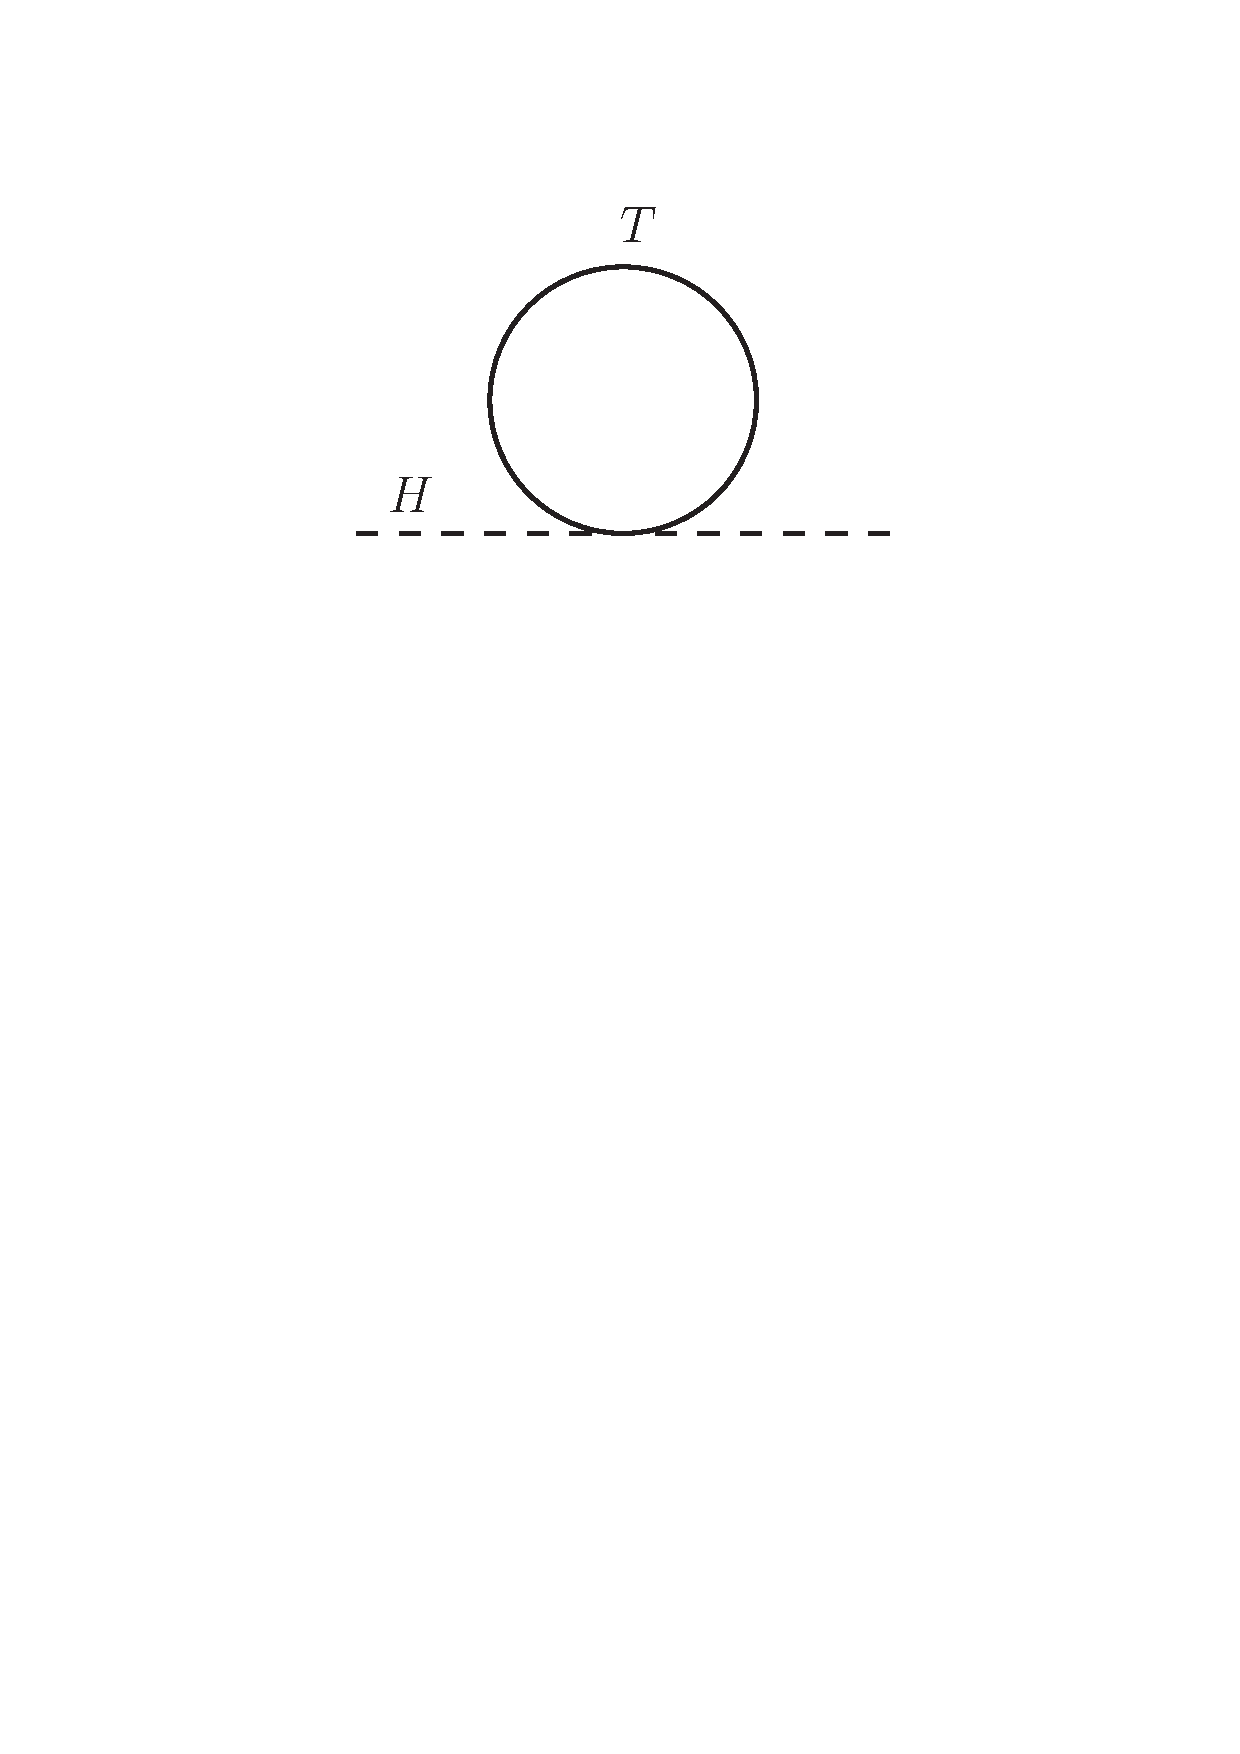
\includegraphics[width=0.92\textwidth]{Theory/FeynmanGraphs/loop_T_good}
    \caption{} \end{subfigure}
	\caption{One-loop contributions to the Higgs boson mass term from (a) the top quark and (b,c) a vector-like top partner.}
          \label{fig:VLQ_loop}
\end{center}
\end{figure}

These new particles can appear as $SU(2)_L$ singlets, doublets or triplets. Their naming and charges is shown in table~\ref{tab:VLQ_tuples}.
\begin{table}[tb]
  \centering
  \begin{minipage}{.4\textwidth}
    \begin{tabular}{cc}
      \toprule
      \toprule
      \textbf{VLQ} & \textbf{Electric charge} \\
      \midrule
      X   & +5/3  \\
      T   & +2/3  \\
      B   & -1/3  \\
      Y   & -4/3  \\
      \bottomrule
      \bottomrule
    \end{tabular}
  \end{minipage}
  \begin{minipage}{.4\textwidth}
    \begin{tabular}{cc}
      \toprule
      \toprule
      \textbf{Multiplet} & \textbf{Hypercharge} \\
      \midrule
      \multicolumn{2}{c}{ Singlets } \\
      $\left(T     \right)$   & $+2/3$  \\
      $\left(B     \right)$   & $-1/3$  \\
      \midrule
      \multicolumn{2}{c}{ Doublets } \\
      $\left(X,T   \right)$   & $+7/6$  \\
      $\left(T,B   \right)$   & $+1/6$  \\
      $\left(B,Y   \right)$   & $-5/6$  \\
      \midrule
      \multicolumn{2}{c}{ Triplets } \\
      $\left(X,T,B \right)$   & $+2/3$  \\
      $\left(T,B,Y \right)$   & $-1/3$  \\
      \bottomrule
      \bottomrule
    \end{tabular}
  \end{minipage}
  \caption{Charge and hypercharge assignment for vector-like quarks in different $SU(2)$ representations.}
  \label{tab:VLQ_tuples}
\end{table}
A mass term for vector-like quarks can be directly inserted into the Lagrangian without breaking the gauge symmetry, so these quarks are also unique in that their coupling to the Higgs field is unrelated to their mass. Therefore there are no constraints on the existence of vector-like quarks arising from the measured Higgs boson production \xsec, since the contribution to loop-induced Higgs boson couplings, $ggH$ and $\gamma\gamma H$, is suppressed by the heavy quark mass.

\subsubsection{Production}
Vector-like quarks can be pair-produced via QCD interactions, or singly produced in association with SM quarks via electroweak interactions. 
The process of pair production through QCD interactions is completely analogous to pair production of SM top quarks, and only depends on \alphas\ and the mass of the heavy quark:
\begin{equation*}
  gg, q\bar{q} \rightarrow Q\bar{Q},\quad \text{with}\ Q = T,B,X,Y .
  \label{VLQ_pairproduction}
\end{equation*}
Single production via electroweak interaction is subdominant for masses below $m_Q \sim 800 - 1000 \gev$, but becomes important for higher masses due to phase-space suppression of pair production. It also depends on the couplings between the new quarks and the $W$ and $Z$ bosons~\cite{Atre:2011ae,Aguilar-Saavedra:2013qpa}:

\begin{equation*}
  qq' \xrightarrow{V^*} qQ,\quad \text{with}\ V = W,Z .
  \label{VLQ_singlepairproduction}
\end{equation*}

\begin{figure}[tb!]
  \centering
  \begin{subfigure}{0.35\textwidth}
    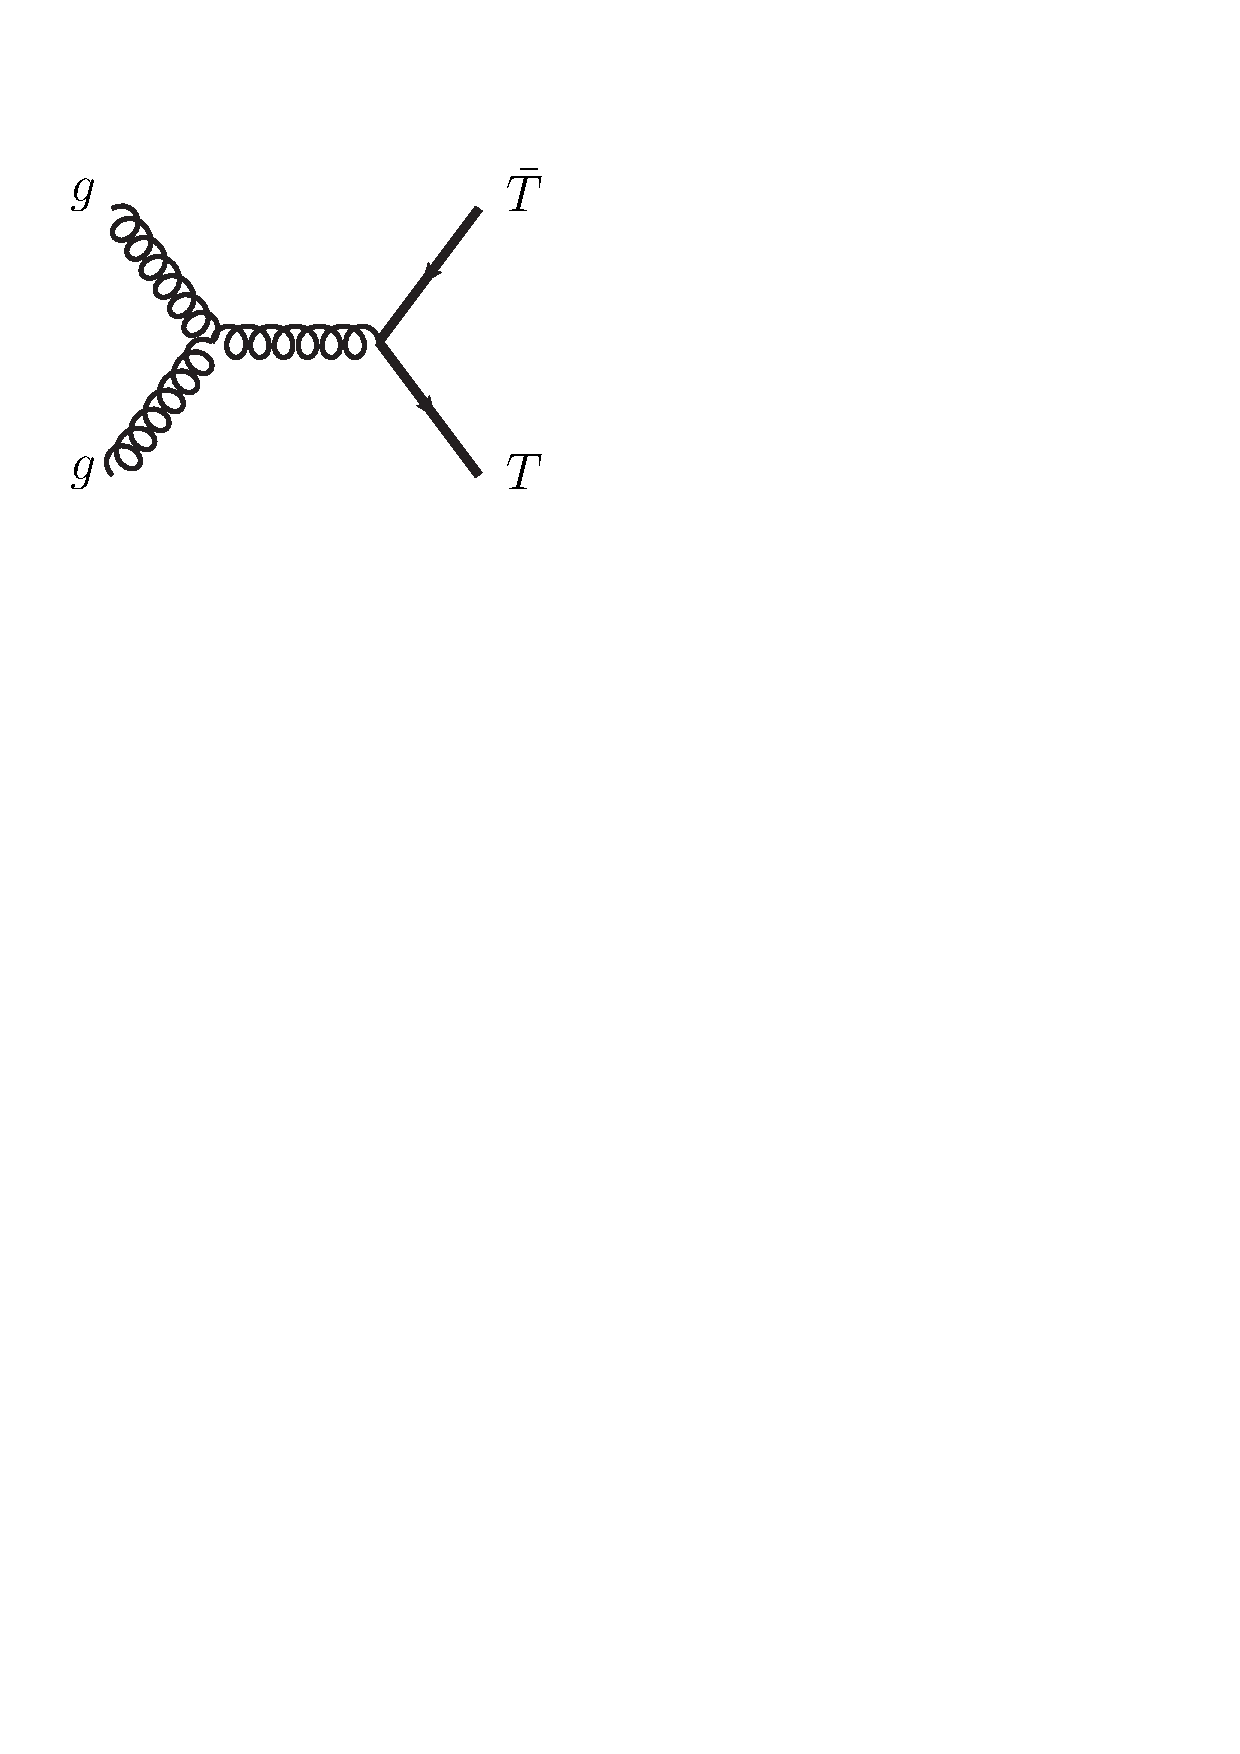
\includegraphics[width=\textwidth]{Theory/FeynmanGraphs/T_pairProd_good.pdf}
  \caption{}
  \label{fig:T_pairProd_good}
\end{subfigure}
  \begin{subfigure}{0.35\textwidth}
    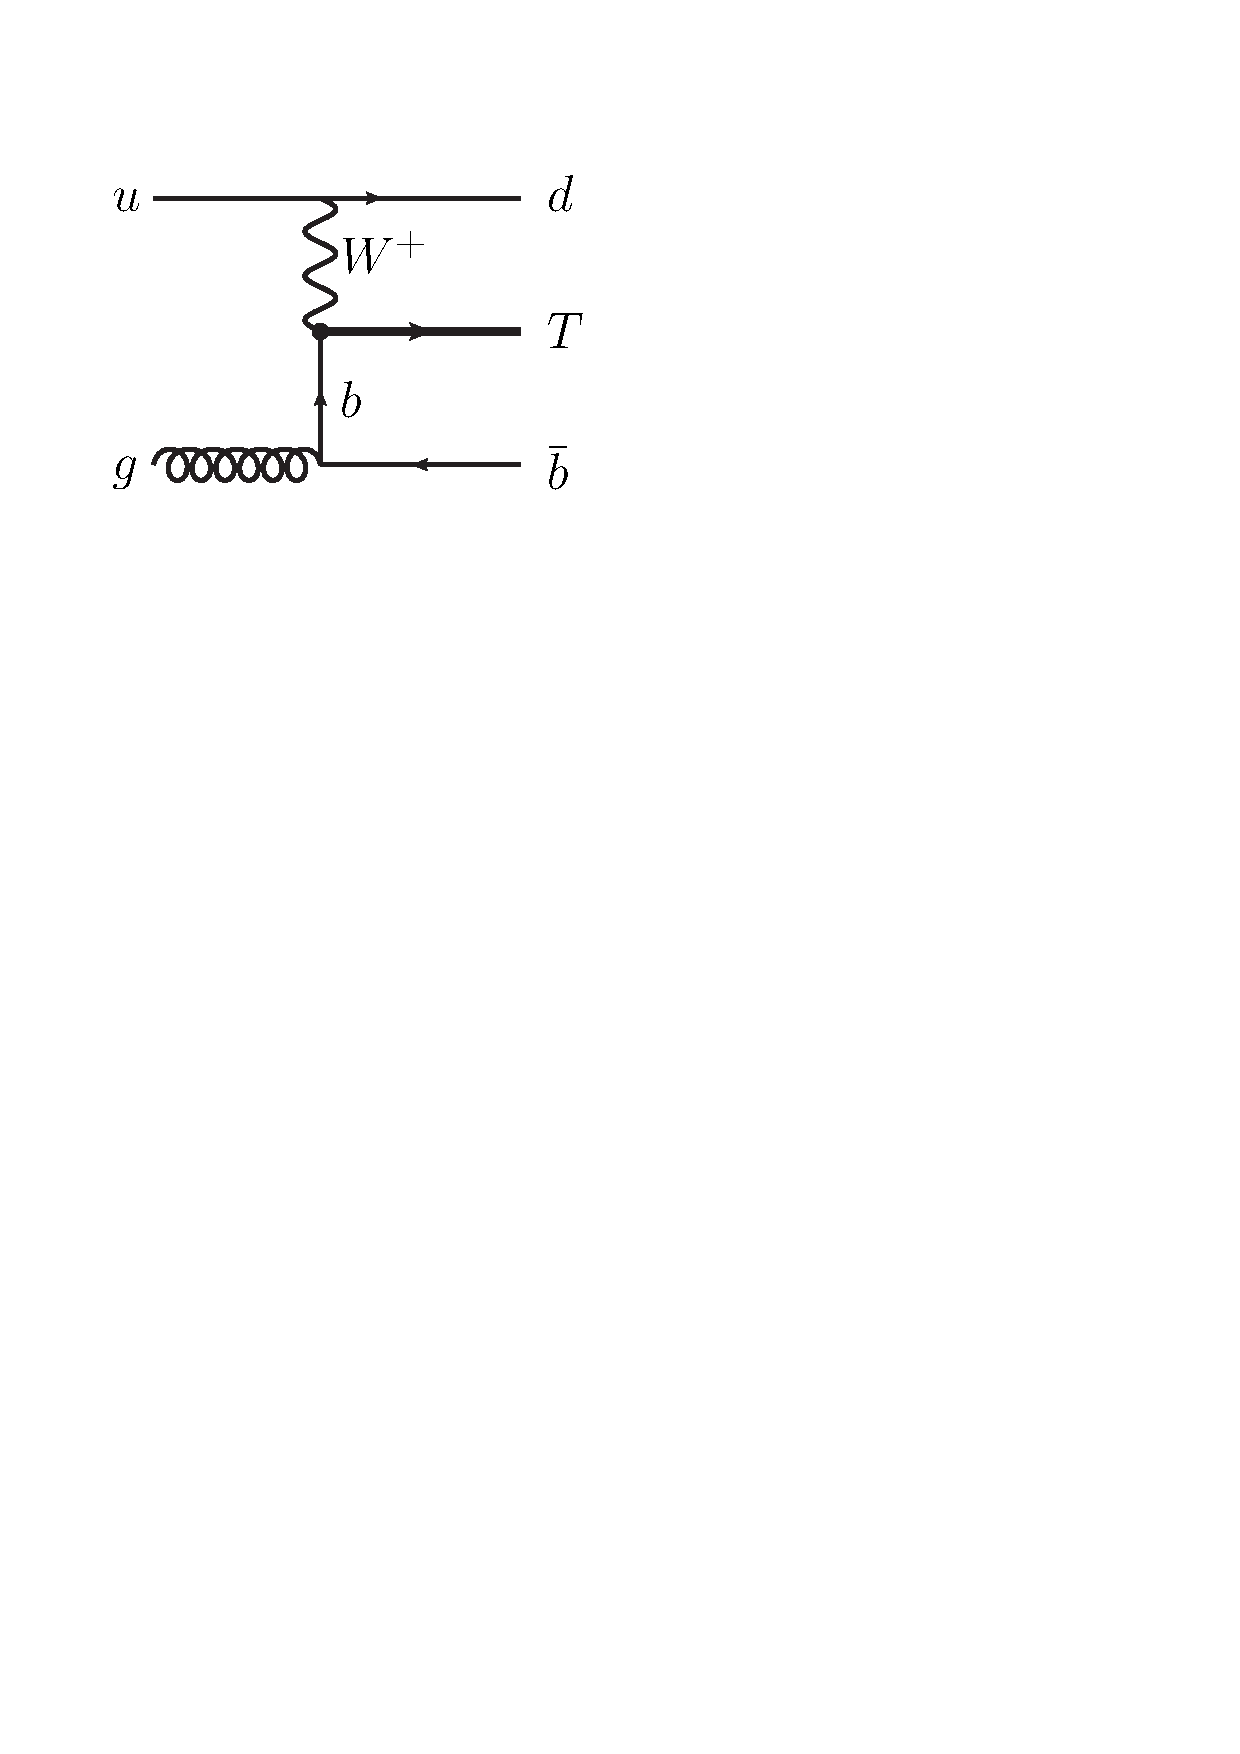
\includegraphics[width=\textwidth]{Theory/FeynmanGraphs/T_singleProd_good.pdf}
  \caption{}
  \label{fig:T_singleProd}
\end{subfigure}
\caption{Example Feynman diagrams for (a) pair production of vector-like top quarks and (b) single production of a vector-like top quark.}
  \label{fig:T_Prod}
\end{figure}

Example Feynman diagrams for pair and single production of vector-like quarks are shown in figure~\ref{fig:T_Prod}.
Figure~\ref{fig:VLQ_production} shows the \xsec\ for pair production and single production in the $t$-channel versus the mass of the vector-like quarks. For a given value of the mass the coupling is set to the maximum allowed by indirect constraints~\cite{Aguilar-Saavedra:2013qpa}.

\begin{figure}[bt!]
  \centering
  \includegraphics[width=0.55\textwidth]{Theory/Figures/VLQ_production.eps}
\caption{Production \xsec\ for heavy quarks  in \pp\ collisions at $\sqrt{s}=\unit[8]{\tev}$ as a function of their mass, for pair production and for single production in different channels.}
  \label{fig:VLQ_production}
\end{figure}

\subsubsection{Decay}
Vector-like quarks decay through electroweak interactions into SM particles. In a general scenario the allowed decays are:

\begin{align*}
  T &\rightarrow W^+b, Zt, Ht \\
  B &\rightarrow W^-t, Zb, Hb \\
  X &\rightarrow W^+t \\
  Y &\rightarrow W^-b~. \\
  \label{VLQ_decays}
\end{align*}

Vector-like quarks can decay via flavor-changing neutral currents since they break the GIM mechanism~\cite{PhysRevD.2.1285}. 
In order to be consistent with precision electroweak data, a small mass splitting between vector-like quarks belonging to the same $SU(2)$ multiplet is required~\cite{Aguilar-Saavedra:2013qpa}, which forbids cascade decays such as $T \to WB$, and leaves direct decays into SM particles as the only possibility. 
In general, the new quarks are expected to couple mainly to the third generation since the mixing of the vector-like quarks with SM quarks is of order $m/M$, where $m$ and $M$ are the masses of the SM quarks and the new quarks respectively~\cite{delAguila:1982fs}.
Couplings to lighter generations, although not favored, are not excluded and can lead to flavor-changing neutral top interactions~\cite{delAguila:1998tp}.

 For the isospin singlets \T\ and \B\ all three decays are possible. However, the scenario is different for the isospin doublets. In the case of a $\left(T, B\right)$ doublet, the two quarks are almost degenerate in mass and the decays strongly depend on the mixing factors of the extended CKM matrix $V_{Tb}$ and $V_{tB}$. If $V_{Tb} \sim V_{tB}$ then the \T\ and \B\ quarks have the same decays as the corresponding singlets but different angular distributions since only the right-handed component of $\left(T, B\right)$ couples to the SM quarks. 
 In the most natural case where $V_{Tb} \muchless V_{tB}$, then the mixing of the heavy quarks with the SM top quark is much stronger, and the $\T \rightarrow Wb$ decay is suppressed, as well as $\B \rightarrow Hb$ and $\B \rightarrow Zb$. This scenario, $V_{Tb} \muchless V_{tB}$, will be assumed throughout this dissertation. Table~\ref{tab:VLQ_decay} summarizes the possible decays of vector-like quarks.

 \begin{table}[b!]
   \centering
   \begin{tabular}{ccc}
   \begin{tabular}{cc}
     \toprule
     \toprule
     Singlets & Decay modes \\
     \midrule
     & \\
     $X$ & $W^+t$ \\
     & \\
     $T$ & $W^+b,\, Ht,\, Zt$ \\
     & \\
     $B$ & $ W^-t,\, Hb,\, Zb$ \\
     & \\
     $Y$ & $W^-b$ \\
     & \\
     & \\%one empty line
     \bottomrule
     \bottomrule
   \end{tabular}

   & 

   \begin{tabular}{cc}
     \toprule
     \toprule
      Doublets & Decay modes\\
     \midrule
     &\\%one empty line
     \multirow{2}{*}{$\left(\begin{array}{c}X \\ T\end{array}\right)$} & $W^+t$\\
     & $Ht,\, Zt$\\
     &\\
     \multirow{2}{*}{$\left(\begin{array}{c}T \\ B\end{array}\right)$} & $ Ht,\, Zt$ \\%$W^+b,\, Ht,\, Zt$\\
     & $ W^-t$\\%$ W^-t,\, Hb,\, Zb$\\
     & \\
     \multirow{2}{*}{$\left(\begin{array}{c}B \\ Y\end{array}\right)$} & $Hb,\, Zb$\\
     & $W^-b$\\
     &\\%one empty line
     \bottomrule
     \bottomrule
   \end{tabular}
   & 

   \begin{tabular}{cc}
     \toprule
     \toprule
      Triplets & Decay modes\\
     \midrule
     &\\%one empty line
     \multirow{3}{*}{$\left(\begin{array}{c}X \\ T \\ B\end{array}\right)$} & $ W^+t$ \\
     & $W^+b,\, Ht,\ Zt$\\
     & $Hb,\, Zb$\\
     &\\%one empty line
     \multirow{3}{*}{$\left(\begin{array}{c}T \\ B \\ Y\end{array}\right)$} & $Ht,\, Zt$\\
     & $W^-t,\, Hb,\, Zb$\\
     & $W^-b$\\
     &\\%one empty line
     &\\%one empty line
     \bottomrule
     \bottomrule
   \end{tabular}
   \end{tabular}
   \caption{Allowed decay modes for vector-like singlets, doublets and triplets.}
     \label{tab:VLQ_decay}
   \end{table}

 The branching ratios of the vector-like quarks depend on the model but also on the heavy quark mass.
 Figure~\ref{fig:VLQ_BR} shows the decay branching ratios of the vector-like top and bottom partners for isosinglets and isodoublets as a function of the heavy-quark mass.

 \begin{figure}
   \centering
   \begin{subfigure}{0.49\textwidth}
     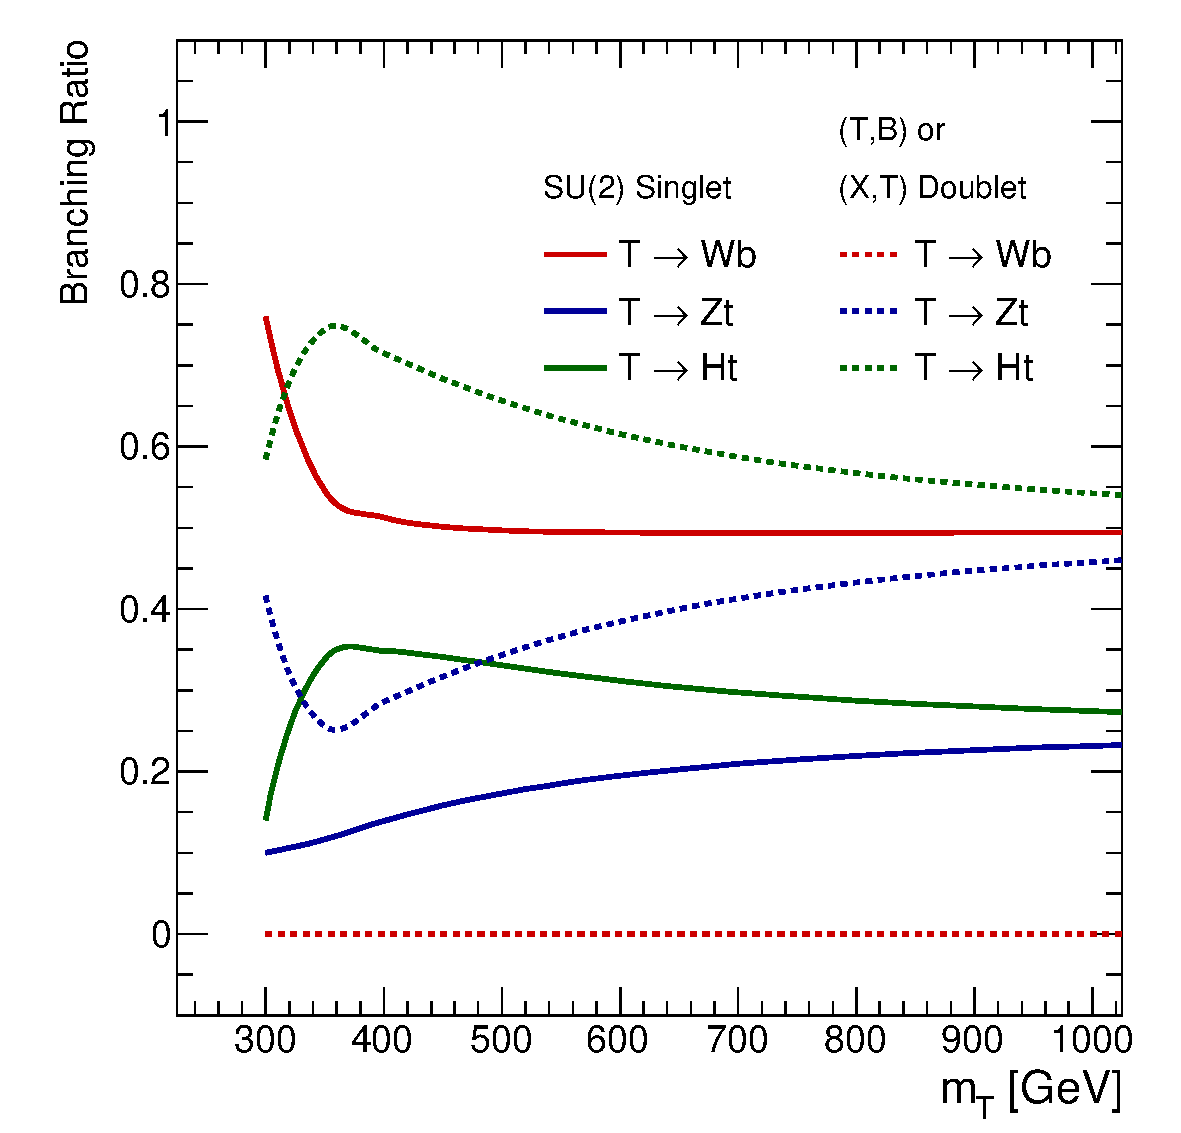
\includegraphics[width=\textwidth]{Theory/Figures/fig_02a.pdf}
     \label{fig:vltbrs}
     \caption{}
 \end{subfigure}
   \begin{subfigure}{0.49\textwidth}
     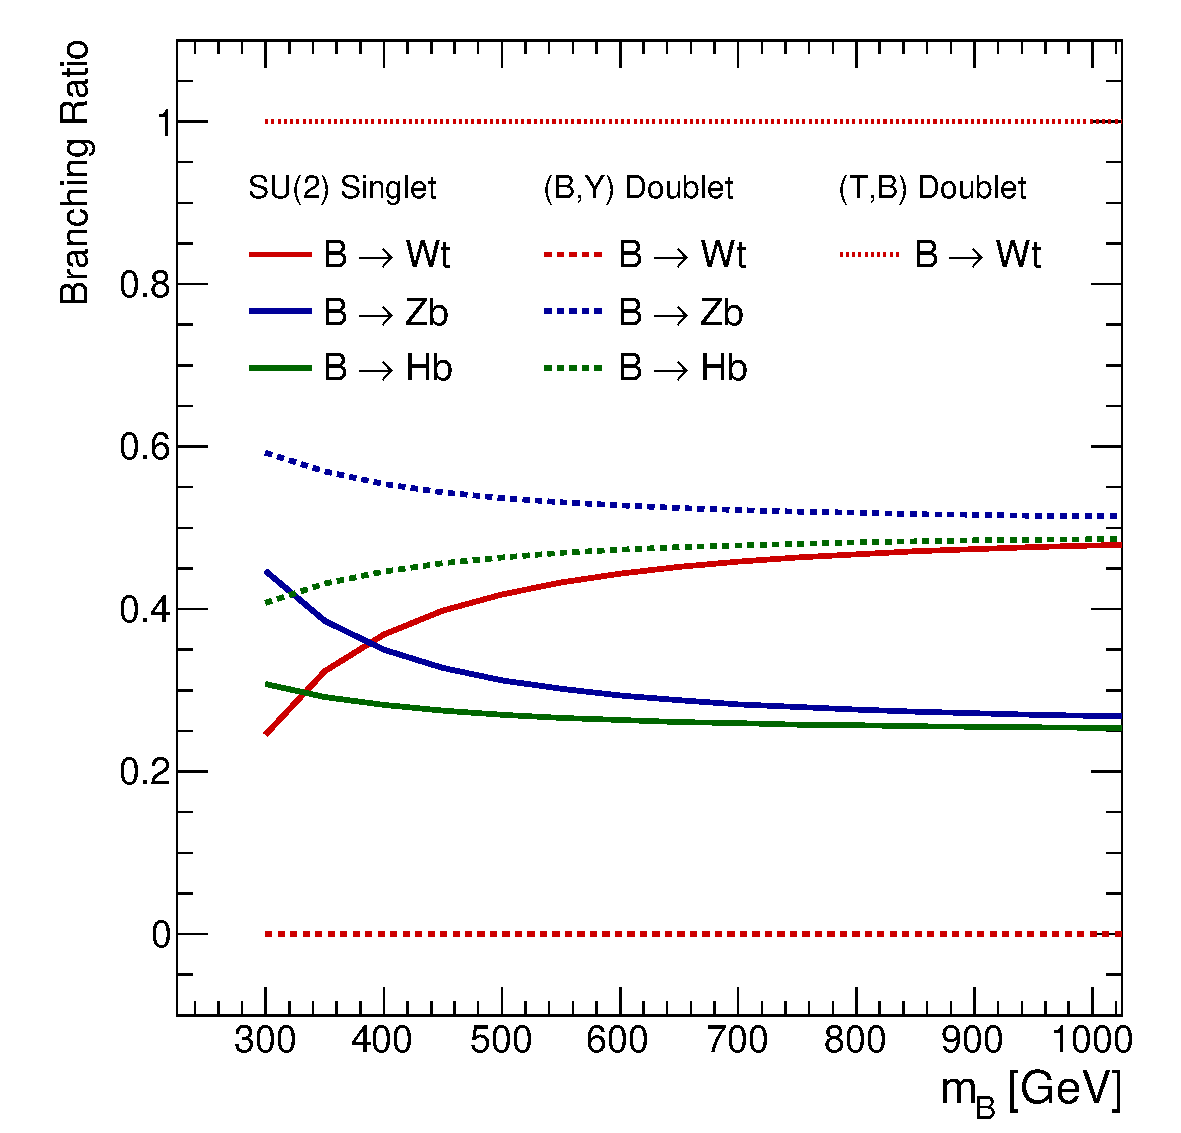
\includegraphics[width=\textwidth]{Theory/Figures/fig_02b.pdf}
     \label{fig:vlbbrs}
     \caption{}
 \end{subfigure}
     \caption{Branching ratio of vector-like top (a) and bottom (b) partners as a function of the heavy quark mass $m_T$ and $m_B$ respectively for isosinglets and isodoublets.}
   \label{fig:VLQ_BR}
 \end{figure}

 After pair production, the decay of at least one vector-like top into a Higgs boson and a top quark produces, following the dominant $H\to b\bar{b}$ decay, a \ttbar-like final state with additional heavy-flavor jets, which is the final state targeted in this dissertation.

\subsection{Bosonic top partners: stops}
The inclusion of bosonic partners of the top quark ($\tilde{t}$, stops) prevents the unnatural fine-tuning
of the Higgs mass, provided that the stops have masses not too far above the weak scale and typically below \unit[1]{\tev}.

Searches for $\st_1$ pair production are challenging because the \xsec\ is 
significantly smaller than for $t\bar{t}$ production (about a factor of six lower for 
$m_{\st_1}\sim m_t$) and the \xsec\ decreases rapidly with increasing $m_{\st_1}$. Direct
searches for $\st_1$ pair production are particularly sensitive in the regime where
$m_{\st_1}\gg m_t + m_{\neut}$, giving rise to signatures with large $\met$ that allow to
distinguish the signal from the $t\bar{t}$ background. 
However, those searches have very limited sensitivity in the kinematic region where $m_{\st_1}\sim m_t + m_{\neut}$, 
given the very similar kinematic features between signal and background. In this scenario,
other strategies need to be pursued to identify topologies with increased separation between
signal and background. One possibility is to search for pair production of
the heavier stop quark, $\st_2$, with subsequent decay $\st_2 \to Z\st_1$, $H\st_1$ and
$t \neut$. This decay chain results in final states with associated production of $t\bar{t}$ with one or more boson ($Z$ or $H$)\footnote{
 For consistency with the other analyses, the capital letter $H$ is used to denote the light Higgs boson. 
 In supersymmetric models the capital letter is commonly used to denote the heavier Higgs boson, while the lowercase $h$ is used to refer to the lighter mass eigenstate which is identified with the \unit[125]{\gev} state discovered at the LHC. Throughout the text, the \unit[125]{\gev} Higgs boson will be denoted by the capital letter $H$ regardless of the model being studied.
},
which provide additional handles to suppress the background. 
In particular the decay through a Higgs boson, and the subsequent $H \to \bbbar$ decay results in a \ttbar\ final state with additional heavy-flavor jets. %Some contribution from decays through a $Z$ boson with $Z \to \bbbar$ is also expected.

For the analysis described in this dissertation, a simplified SUSY model is considered where only the top quark partners and the lightest neutralino, \stopone, \stoptwo, \neutralino, are considered to be kinematically accessible at the LHC. The masses for the rest of the SUSY spectrum are set arbitrarily high. Therefore, production and decay processes involving other SUSY particles such as $\gluino \to \stopone t$ or $\stopone \to \chinoonepm b$ are not considered.

\subsubsection{Production}

\begin{figure}[!tb]
\begin{center}
\mbox{
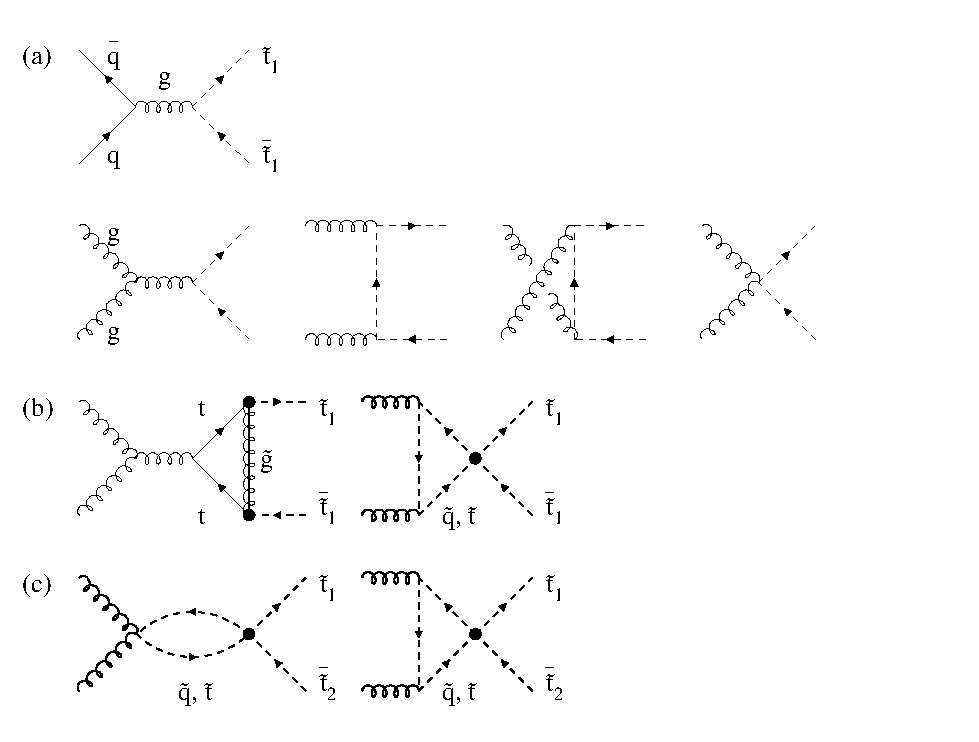
\includegraphics[trim=0.8cm 5.7cm 0cm 0cm, clip=true, width=0.995\textwidth]{Theory/Figures/feyn_fin.eps}
}
\end{center}
\caption{Born diagrams for quark-antiquark annihilation and gluon fusion, leading to pairs of stop pair production.}
\label{fig:StopProductionDiagrams}
\end{figure}

At hadron colliders, stop pairs can be produced at leading order in quark-antiquark annihilation and gluon-gluon fusion:

\begin{equation}
\begin{matrix}
q \bar{q} \rightarrow & \stopone \antistopone, & \stoptwo \antistoptwo~,\\
gg        \rightarrow & \stopone \antistopone, & \stoptwo \antistoptwo~,\\
\end{matrix}
\label{eq:DirectStopSbottomProduction}
\end{equation}
and the relevant leading order diagrams for these processes are found in figure~\ref{fig:StopProductionDiagrams}.
The production of \stopone\ and \stoptwo\ pairs is completely identical and depends only on $\alphas$ and the mass of the particle. Although the analysis presented in this dissertation targets the pair production of \stoptwo, the process of \stopone\ pair production is also present in the simplified model and has to be taken into account. 
The production of mixed \stopone \antistoptwo\ or \stoptwo \antistopone\ pairs is suppressed as the \xsec\ is of order $\alphas^4$ and will not be considered~\cite{Beenakker:1997ut}.

\subsubsection{Decay}
The possible decays of the stop particles are limited within the simplified SUSY model:
\begin{align*}
  \stopone &\to t \neutralino \\
  \stoptwo &\to t \neutralino, ~\stopone H, ~\stopone Z, 
  \label{eq:stop_decay}
\end{align*}
and the \neutralino\ is considered the LSP and is therefore stable.

The branching fractions to the three possible decays of the \stoptwo\ are not predicted by the model and will be considered free parameters. In the parameter region where $m_{\stoptwo} < m_{\stopone} + m_H$, the decay through a Higgs boson is suppressed. If $m_{\stoptwo} < m_{\stopone} + m_Z$, only the decay to a top quark and neutralino is possible. Figure~\ref{fig:stop_decay} shows two examples of \stoptwo\ decays to the different allowed particles.

\begin{figure}[tb!]
  \centering
  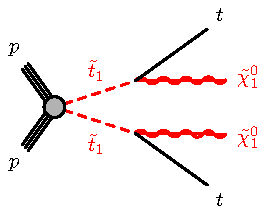
\includegraphics[width=0.32\textwidth]{Theory/FeynmanGraphs/FeynmanGraphsSUSY/stst-ttN1N1.eps}
  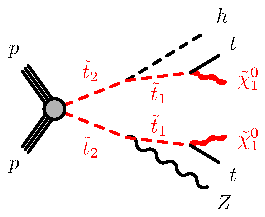
\includegraphics[width=0.32\textwidth]{Theory/FeynmanGraphs/FeynmanGraphsSUSY/st2st2-ZhttN1N1.eps}
  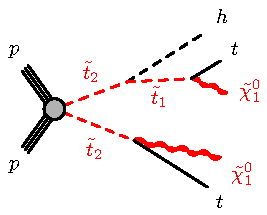
\includegraphics[width=0.32\textwidth]{Theory/FeynmanGraphs/FeynmanGraphsSUSY/st2st2-httN1N1.eps}
  \caption{Examples of decays of \stopone\ and \stoptwo\ particles in the different allowed decay channels.}
  \label{fig:stop_decay}
\end{figure}

\subsection{Four-top-quark production}
The production rate of four-top-quark events is very small in the SM, with a \xsec\ of $\sigma_\fourtop \approx \unit[1]{fb}$ at $\sqrt{s}=\unit[8]{\tev}$~\cite{Barger:1991vn,Barger:2010uw}. However many BSM theories predict an increase of this final state, usually through the pair production of a new particle decaying to a top-antitop pair. The subsequent decay produces a spectacular final state which, in the case of one leptonic $W$ decay, produces up to ten jets with four of them originating from $b$-quarks.
Figure~\ref{fig:fourtop_FD} depicts representative LO Feynman diagrams for four-top-quark production within the SM and the BSM scenarios considered in this dissertation. 

The phenomenology of the different models predicting an increase of the four-top-quarks final state is discussed in the following.

\begin{figure}[tbp]
\centering
\begin{subfigure}{0.49\textwidth} 
\centering
  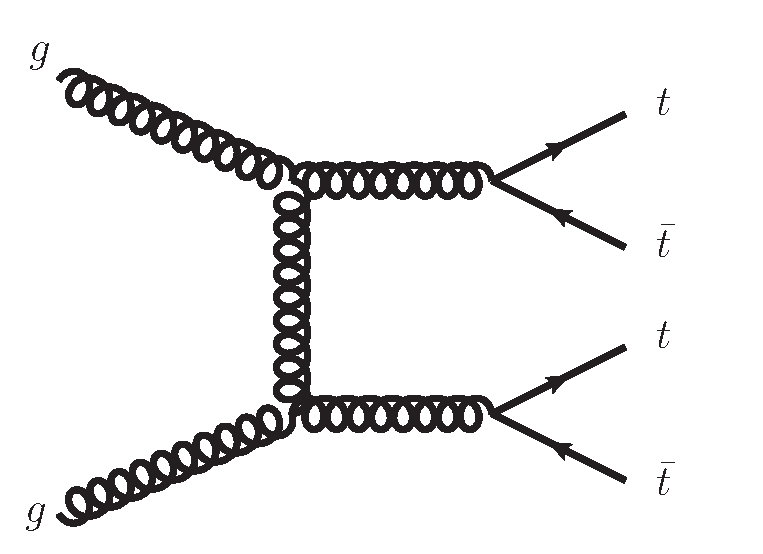
\includegraphics[width=0.66\textwidth]{Theory/FeynmanGraphs/4tops_SM.eps}
  \caption{}\label{fig:fourtop_SM} \end{subfigure}
\begin{subfigure}{0.49\textwidth} 
\centering
  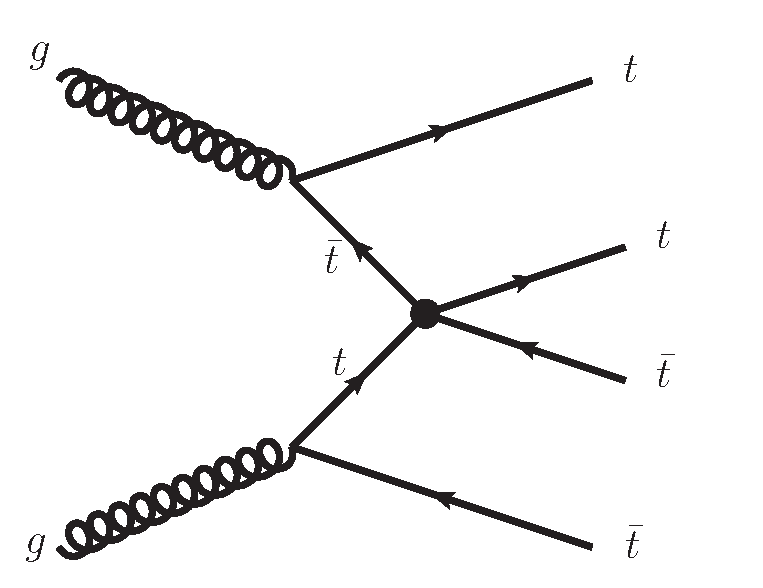
\includegraphics[width=0.60\textwidth]{Theory/FeynmanGraphs/4tops_CI.eps}
  \caption{}\label{fig:fourtop_CI} \end{subfigure}
\\
\begin{subfigure}{0.49\textwidth} 
\centering
  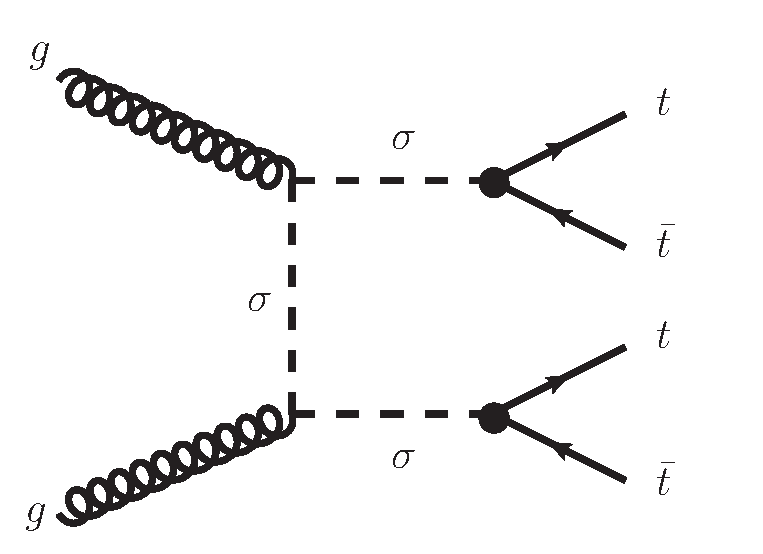
\includegraphics[width=0.66\textwidth]{Theory/FeynmanGraphs/4tops_sgluon.eps}
  \caption{}\label{fig:fourtop_sgluon} \end{subfigure}
\begin{subfigure}{0.49\textwidth} 
\centering
  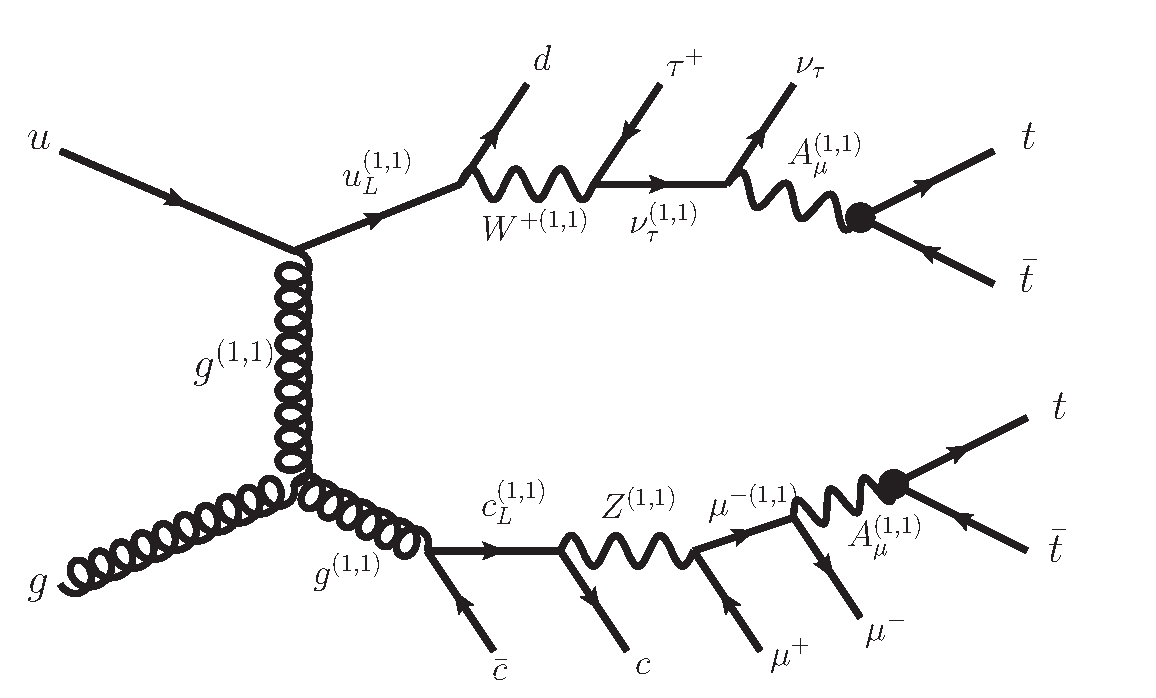
\includegraphics[width=0.80\textwidth]{Theory/FeynmanGraphs/4tops_UEDRPP.eps}
  \caption{}\label{fig:fourtop_UEDRPP} \end{subfigure}
\caption{Representative leading-order Feynman diagrams for four-top-quark production within (a) the SM 
and several BSM scenarios: (b) via an effective four-top-quark interaction in an effective field theory 
model, (c) via scalar-gluon-pair production, and (d) via cascade decays from Kaluza-Klein excitations in an universal extra dimensions 
model with two extra dimensions compactified under the real projective plane. }
\label{fig:fourtop_FD}
\end{figure}

\subsubsection{Kaluza-Klein modes}
\label{subsubsec:KKmodes}
In the model with two universal extra dimensions discussed in section~\ref{subsubsec:UED}, gauge bosons propagating in the extra dimensions produce a tower of KK vector modes. The compactification of the two extra dimensions under the real projective plane geometry (2UED/RPP) leads to the discretization of the momenta along these directions. The set of solutions of the field equation are described by two integers $(j,k)$, referred to as KK numbers. A \textit{tier} $(j,k)$ is the set of particles with same KK numbers. At leading-order the masses of the particles within a tier $(j,k)$ are: 
\begin{equation}
  m^2 = \frac{j^2}{R^2_4}+\frac{k^2}{R^2_5}~, 
  \label{eq:tier_masses}
\end{equation}
where $\pi R_4$ and $\pi R_5$ are the size of the two extra dimensions.
The model is parameterized by $R_4$ and $R_5$ or, alternatively, by 
$m_{\KK}=1/R_4$ and $\xi=R_4/R_5$. 
Particles from the level-1 modes ($j+k=1$)  would decay into soft leptons and jets plus missing energy~\cite{Cheng:2002ab}, making their discovery challenging. However, level-2 modes can be produced at colliders, their decay into level-1 modes is kinematically forbidden and have large branching fractions for decays into a pair of SM particles. 

Four-top-quark production can arise from tier $(1,1)$, where particles
from this tier have to be pair produced because of symmetries of the model. Then they chain-decay to the 
lightest particle of this tier, the heavy photon $A^{(1,1)}$, by emitting SM particles (see figure~\ref{fig:fourtop_UEDRPP}). 
The branching ratios of $A^{(1,1)}$ into SM particles are not predicted by the model, although the decay 
into $\ttbar$ is expected to be dominant~\cite{Cacciapaglia:2011kz}. Four-top-quark events can also arise from 
tiers $(2,0)$ and $(0,2)$ via a similar mechanism. In this case the expected \xsec\ for four-top-quark production 
is reduced compared to that from tier $(1,1)$ since each state in tiers $(2,0)$ and $(0,2)$ can decay 
directly into a pair of SM particles or into a pair of states in tiers $(1,0)$ or $(0,1)$ via bulk interactions, 
resulting into smaller branching ratios for decay into $t\bar{t}$~\cite{Cacciapaglia:2011kz}.
In the following, when considering four-top-quark production from a given tier, it will be
assumed that the $A$ photon in that tier decays with 100\% branching ratio into $\ttbar$ 
while $A$ photons from other tiers cannot decay into $\ttbar$.

Due to the geometry of the space an $SO(2)$ symmetry arises, usually referred to as KK parity. This symmetry forbids the decay of the lightest particle from tier $(1,0)$ (and tier $(0,1)$ in case of equal radii) to SM particles, thus allowing for a natural dark matter candidate~\cite{Cheng:2002ej,Servant:2002aq}. 
Observations of dark matter relic abundance favor values of $m_{\KK}$ between $600\gev$ and $1200\gev$~\cite{Arbey:2012ke}.

\subsubsection{Sgluons}
Scalar particles, which are color-octets, are predicted in several models and are usually referred to as \textit{sgluons}. Some supersymmetric models consider Dirac gauginos~\cite{Plehn:2008ae,Choi:2008ub}, which have a corresponding scalar in the adjoint representation of QCD, and SM-like R-parity.
Sgluon particles are also predicted in non-supersymmetric models~\cite{Kilic:2009mi,Kilic:2008pm,Burdman:2006gy,Calvet:2012rk} such as extra-dimension models and models with a new strong sector leading to scalar pseudo-Goldstone bosons which can be identified with the sgluons.

Once produced through standard strong interactions, a sgluon can decay either to a quark pair or to a gluon pair.
For sgluon masses above twice the top-quark mass, the dominant decay mode is into \ttbar, giving rise to a four-top-quark final state (figure~\ref{fig:fourtop_sgluon}). 
For the analysis described in this dissertation a \unit[100]{\%} branching ratio to top quarks is considered.

\subsubsection{Contact interactions}
The four-top-quarks signatures described in previous sections assume the pair-production of a new particle that can be produced at the LHC.
However when the mass of the new particle is beyond the energy reach of the LHC, its effect on different observables can still be noticeable. An effective field theory (EFT) formalism can be used, where the effect of new physics is described by non-renormalizable operators of higher order~\cite{Degrande:2010kt}. An operator for four-top-quarks contact interaction (see figure~\ref{fig:fourtop_CI}) can be considered:
\begin{equation}
  \lagrangian_{4t} = \frac{C_{4t}}{\Lambda^2}(\bar{t}_R \gamma^\mu t_R)(\bar{t}_R \gamma_\mu t_R)~.
  \label{eq:contact_interaction}
\end{equation}
Only the contact interaction operator with right-handed top quarks is considered as left-handed top quark operators are already strongly constrained by electroweak precision data~\cite{Georgi:1994ha}.

This approach can be used to parameterize composite top quark scenarios~\cite{Pomarol:2008bh,Kumar:2009vs,Lillie:2007hd}, with a new strongly interacting sector or new heavy vector particles predicted in Randall-Sundrum theories~\cite{Guchait:2007jd}.
